% Bodies Are Stable, Behaviour Is Not
% Gursahib Singh, Gregory S. Anderson (Thompson Rivers University)
% Constraint: no em dashes anywhere in the body.
% Every number in this file is produced by src/ and checked by 09_verify_paper.py

\documentclass[conference]{IEEEtran}
\usepackage{cite}
\usepackage{amsmath,amssymb,amsfonts}
\usepackage{graphicx}
\usepackage{textcomp}
\usepackage{booktabs}
\usepackage[hidelinks]{hyperref}
\usepackage{url}
\Urlmuskip=0mu plus 1mu\relax
\usepackage{stfloats}
\usepackage{placeins}
\usepackage{array}
\usepackage{balance}

\setcounter{topnumber}{3}
\setcounter{bottomnumber}{2}
\setcounter{totalnumber}{5}
\renewcommand{\topfraction}{0.92}
\renewcommand{\bottomfraction}{0.75}
\renewcommand{\textfraction}{0.06}
\renewcommand{\floatpagefraction}{0.70}
\renewcommand{\dblfloatpagefraction}{0.70}
\renewcommand{\dbltopfraction}{0.92}
\setcounter{dbltopnumber}{3}

\graphicspath{{../outputs/plots/}}

\begin{document}

\title{Bodies Are Stable, Behaviour Is Not:\\
A Personalization Ladder for Health and\\
Fitness Recommendation}

\author{
\IEEEauthorblockN{Gursahib Singh}
\IEEEauthorblockA{\textit{Department of Computing Science}\\
\textit{Thompson Rivers University}\\
Kamloops, BC, Canada}
\and
\IEEEauthorblockN{Gregory S. Anderson}
\IEEEauthorblockA{\textit{Dean, Faculty of Science}\\
\textit{Thompson Rivers University}\\
Kamloops, BC, Canada}
}

\maketitle

%========================================
\begin{abstract}
Health and fitness applications personalize by profile: age, sex, and body mass index. We ask how far that can go. Staged views of personalization depth are not new, running from the mass, targeted, and tailored trichotomy of health communication to a recent six-level scheme for personal health agents. What is missing is the measurement. We take a five-rung ladder, from a population constant (L0) through a demographic lookup (L1), body measurements (L2), the user's own logged behaviour (L3), and continuous context (L4), and score what each rung is worth on real data, in one study, on one cohort, under one metric. The expert-authored engine in the book this work accompanies is an L1 system: across 378 adult user types it emits 14 distinct recommendations, and its activity, sleep, and fluid targets are a single constant for everyone. In NHANES 2013--2014 ($n = 6{,}113$ adults, design-weighted), age, sex, and BMI explain 89.5\% of the variance in waist-to-height ratio but 7.4\% of the variance in physical activity, and adding BMI to age and sex leaves behaviour prediction unchanged to four decimal places in both $R^2$ and AUC. A variance decomposition on 71 people wearing trackers for a median of 88 days explains why: the median intraclass correlation is 0.26 for behaviour and 0.57 for physiology, so roughly three quarters of what a person does is a property of the day rather than of the person. Out of sample with forward chaining, L0, L1, and L2 all have negative $R^2$ for next-day step count and sit at or below $+0.018$ for active minutes, L3 reaches $+0.226$, and L4 adds $+0.003$; the ordering replicates in a second, independent cohort. For adherence, predicting whether somebody meets their step goal, a static profile reaches AUC 0.604 and the person's own adherence history reaches 0.746, although with 51 participants no adjacent pair of rungs separates from zero. Personalization switches on after one to two days of logging. Because each rung also costs more disclosure, these measurements are a privacy-utility curve, and only one marginal gain is distinguishable from zero: the behaviour log. We caution that our L4 is one operationalization, day-lagged momentary self-report and physiology present on a median of 45\% of days, so its null result bounds that design rather than context-aware intervention in general. We also report, in an appendix, a four-detector battery for fabricated datasets, built because five of the public fitness datasets we screened proved synthetic and a single-column determination test detects only one of them.
\end{abstract}

\begin{IEEEkeywords}
recommender systems, mobile health, physical activity, personalization, within-person variability, adherence, data minimization, dataset quality
\end{IEEEkeywords}

%========================================
\section{Introduction}

A health application knows some things about a user at signup and learns others over time. The signup facts are cheap, permanent, and easy to reason about: age, sex, height, weight. The learned facts are expensive, arrive slowly, and are messy: what the person actually did yesterday, and the day before that. Almost every deployed fitness recommender is built on the first kind.

That choice is reasonable on its face. Public health guidance is written in terms of the first kind, because guidance is written for populations. It is also what a book can use, since a book cannot know what its reader did yesterday.

This paper asks what that choice costs, and answers it in measured quantities rather than in principle. We use a \textit{personalization ladder} of five rungs, each corresponding to a real design decision somebody must make when building such a system, and each requiring strictly more from the user than the one below it:

\begin{itemize}
\item \textbf{L0}, a population constant: one recommendation for everyone.
\item \textbf{L1}, a demographic lookup: a function of age, sex, and a self-reported activity level.
\item \textbf{L2}, plus body measurements: height, weight, waist, BMI.
\item \textbf{L3}, plus the person's own logged behaviour history.
\item \textbf{L4}, plus continuous context: yesterday's mood, place, and physiology.
\end{itemize}

We claim no originality for the ladder itself. Ordered accounts of personalization depth already exist (Section~\ref{sec:depth}), and the rungs below are close to a scheme published as a preprint while this work was in progress \cite{abbasian2025pcu}. What does not exist is a measurement of what each rung is worth, and that is what this paper supplies.

Our baseline is not a strawman. This work accompanies a wellness logbook written by the second author \cite{anderson2026logbook}, which contains an explicit recommendation engine, given as pseudocode, that is an L1 system. Section~\ref{sec:engine} audits it. We find that it is guideline-faithful, safe, and capable of emitting 14 distinct recommendations for the entire adult population. That is not a criticism of the book. It is the structural limit of what a population guideline can express about one person, and it is the gap this paper measures.

\subsection{Contributions}
\begin{enumerate}
\item \textbf{The missing measurement.} Staged accounts of personalization depth grade systems but do not price the grades \cite{tenklooster2024clarifying, matthews2025mentalhealth, alslaity2023panoramic}. On two wearable cohorts and one national survey we score every rung under a single metric. The gain from L1 to L2, the single most obvious improvement a developer would make, is $+0.0004$ in out-of-sample $R^2$. The gain from L2 to L3 is $+0.2429$.
\item \textbf{An explanation, not just a result.} A variance decomposition shows the median intraclass correlation for behaviour is 0.26 against 0.57 for physiology. Static profiles predict the body well and behaviour badly because the body is a person-level trait and behaviour largely is not.
\item \textbf{Adherence as the operative quantity.} We model whether a real step goal is met. The person's own adherence history reaches AUC 0.746 against 0.604 for any static description, an ordering consistent with the rest of the paper though not itself statistically separated at $n = 51$.
\item \textbf{A cold-start answer.} One to two days of logging already beats every static rung, and the curve peaks at two to four weeks.
\item \textbf{A measured privacy-utility curve.} Three of four marginal gains along the ladder are negative. We argue data minimization from evidence rather than from principle.
\item \textbf{A fabrication battery} (Appendix~\ref{app:battery}). Screening candidate training data, we found five synthetic datasets of which a single-column determination test catches one. We give four complementary detectors that catch all five with no false alarms on four real datasets.
\end{enumerate}

%========================================
\section{Related Work}

\subsection{Health and Activity Recommenders}
Recommender systems for physical activity and diet are an active area, catalogued in surveys of health recommender systems \cite{decroon2021hrs, tran2021healthcare} and framed as a research agenda in \cite{schafer2017health}. Most deployed systems personalize on a static profile, including food and diet recommenders \cite{min2020food, elsweiler2022foodrs}. Systems that adapt to a user's own logged behaviour do exist \cite{rabbi2015mybehavior}, and frameworks for user modelling in fitness coaching have been proposed \cite{herrmanny2021umap}. The most methodologically rigorous line of work is the just-in-time adaptive intervention (JITAI) framework \cite{nahumshani2018jitai}, in which decision points, tailoring variables, and proximal outcomes are specified in advance and effects are established through micro-randomized trials \cite{klasnja2015mrt, klasnja2019heartsteps}, with an accompanying methodology for sample size \cite{liao2016samplesize}, time-varying effects \cite{boruvka2018tveffect, qian2021excursion}, and off-policy evaluation \cite{liao2021offpolicy, liao2020personalized}. Our L4 rung is a deliberately simplified stand-in for that framework, and our results speak to when the additional machinery is warranted.

\subsection{Staged Accounts of Personalization Depth}
\label{sec:depth}
Ordering personalization by depth is an old idea. Health communication distinguishes mass, targeted, and tailored messaging \cite{kreuter1999onesize, hawkins2008tailoring}; persuasive systems research separates weak personalization by segment from strong personalization of the individual \cite{oinaskukkonen2022truepers}; recommender surveys cut static from dynamic bases \cite{alslaity2023panoramic}; earlier work separates demographic, content-based, and collaborative sources \cite{pazzani1999framework}, and decomposes personalization into orthogonal facets of what is personalized, for whom, and by whom \cite{fanpoole2006personalization}. In digital health, 61 mental health systems have been graded on an ordinal weak, intermediate, and strong-adaptive scale \cite{matthews2025mentalhealth}, tailoring mechanisms for real-time activity coaching have been catalogued \cite{opdenakker2014tailoring}, and segmentation variables have been organized into categories that the authors deliberately leave unordered \cite{tenklooster2024clarifying}. A six-level scheme for personal health agents, explicitly modelled on the levels of driving automation, was posted as a preprint during this work \cite{abbasian2025pcu}; its levels correspond closely to ours, though it contains no anthropometric rung, and its authors describe the table as illustrative rather than prescriptive and report no data behind it.

We therefore claim no novelty for the structure. We claim the measurement. The reviews above are explicit that it is missing: segmentation variables are analysed together so that it is difficult to draw conclusions about their separate effects \cite{tenklooster2024clarifying}, controlled trials "lacked a non-personalised intervention, making it difficult to determine the added value" \cite{matthews2025mentalhealth}, and personalization bases are ranked by how often they are used rather than by what they are worth \cite{alslaity2023panoramic}.

One objection deserves a direct answer. Hawkins et al.\ \cite{hawkins2008tailoring} argue that these categories are overlapping segments of continua rather than discrete levels, and against a depth scale defined by degree of audience segmentation that is correct. Our rungs are not cut that way. They are cut by the availability of an input class, which for a deployed system is a binary engineering fact: either the application holds that person's own logged history or it does not. That is what makes each rung separately priceable.

\subsection{Within-Person Versus Between-Person Structure}
The distinction we rely on is old and well established outside this application area. Molenaar's argument that group-level structure does not generally transfer to the individual \cite{molenaar2004}, and its empirical confirmation that group-to-individual generalizability fails for many psychological processes \cite{fisher2018pnas}, are the theoretical statement of what we measure here. Intraclass correlation is the standard estimator \cite{shrout1979icc, koo2016icc}, and the day-to-day instability of physical activity is documented in the accelerometry literature \cite{trost2005accel, tudorlocke2005days}. The same logic motivates small-data and N-of-1 designs in health \cite{hekler2019smalldata, lillie2011nof1}, and day-to-day fluctuation in health behaviour is itself an object of study \cite{chevance2021fluctuations}. Our contribution is to carry the argument into recommendation and to price each rung of the resulting design space.

\subsection{The Limits of BMI}
BMI is a population screening statistic that cannot separate fat mass from lean mass \cite{prentice2001bmi, rothman2008bmi, nevill2006bmi}, and the American Medical Association's 2023 policy states that it loses predictability at the individual level \cite{ama2023bmi}. Waist-to-height ratio tracks central adiposity more closely \cite{browning2010whtr, ashwell2016whtr}. We reproduce that ordering and then show that it is beside the point for behaviour: no anthropometric variable we tested helps predict what somebody does.

\subsection{Short-Horizon Activity Prediction}
Forecasting a person's near-term activity has precedent. Fellger et al.\ \cite{fellger2020nextday} predict next-day active minutes at NRMSE 9.11\% with $r = 0.89$. Their folds are subject-wise, but the correlation and the normalized error are computed over predictions pooled across all 44 participants, so both absorb between-person variance and are not within-person figures. We group every split by person \cite{saeb2017usecase} and report a within-person out-of-sample $R^2$ instead. Abdulghani et al.\ \cite{abdulghani2026phenotype} predict next-day steps in three-hour segments at MAE 981, reporting no $R^2$. A related line sets adaptive step goals from a participant's own recent history \cite{adams2013adaptive, korinek2018stepgoals, poirier2016walking, zhou2018stepgoals, adams2022reinforcement}; these rules are implicitly point forecasts, but none reports a forecast-accuracy figure.

We therefore cannot benchmark our $R^2$ against a published within-person out-of-sample value for next-day step count, because we could not find one. We report ours as a comparison between rungs under a fixed protocol, which is what the paper's argument requires, and not as a state-of-the-art claim.

\subsection{Dataset Quality}
Leakage and degenerate targets inflate reported accuracy across applied machine learning \cite{kaufman2012leakage, kapoor2023leakage}, documentation practice remains uneven \cite{gebru2021datasheets}, and the provenance of widely used public health datasets is often unestablishable \cite{gibson2026provenance}. Section~\ref{sec:battery} adds a specific finding: a single-question screen, including our own, misses most fabrication.

%========================================
\section{An Audit of a Deployed Expert Engine}
\label{sec:engine}

The book accompanying this work \cite{anderson2026logbook} specifies a recommendation engine in pseudocode. Food-group servings are a function of age band and sex; daily calories a function of age band, sex, and a self-reported activity level; heart-rate zones a function of age; and activity, sleep, and fluid targets are fixed constants. Nothing a user logs after onboarding enters any of these.

We implemented the engine exactly as written and enumerated its complete output space over a realistic adult input grid of ages 18 to 80, two sexes, and three activity levels, giving 378 distinct user types (Fig.~\ref{fig:outputspace}).

\begin{figure}[t]
\centering
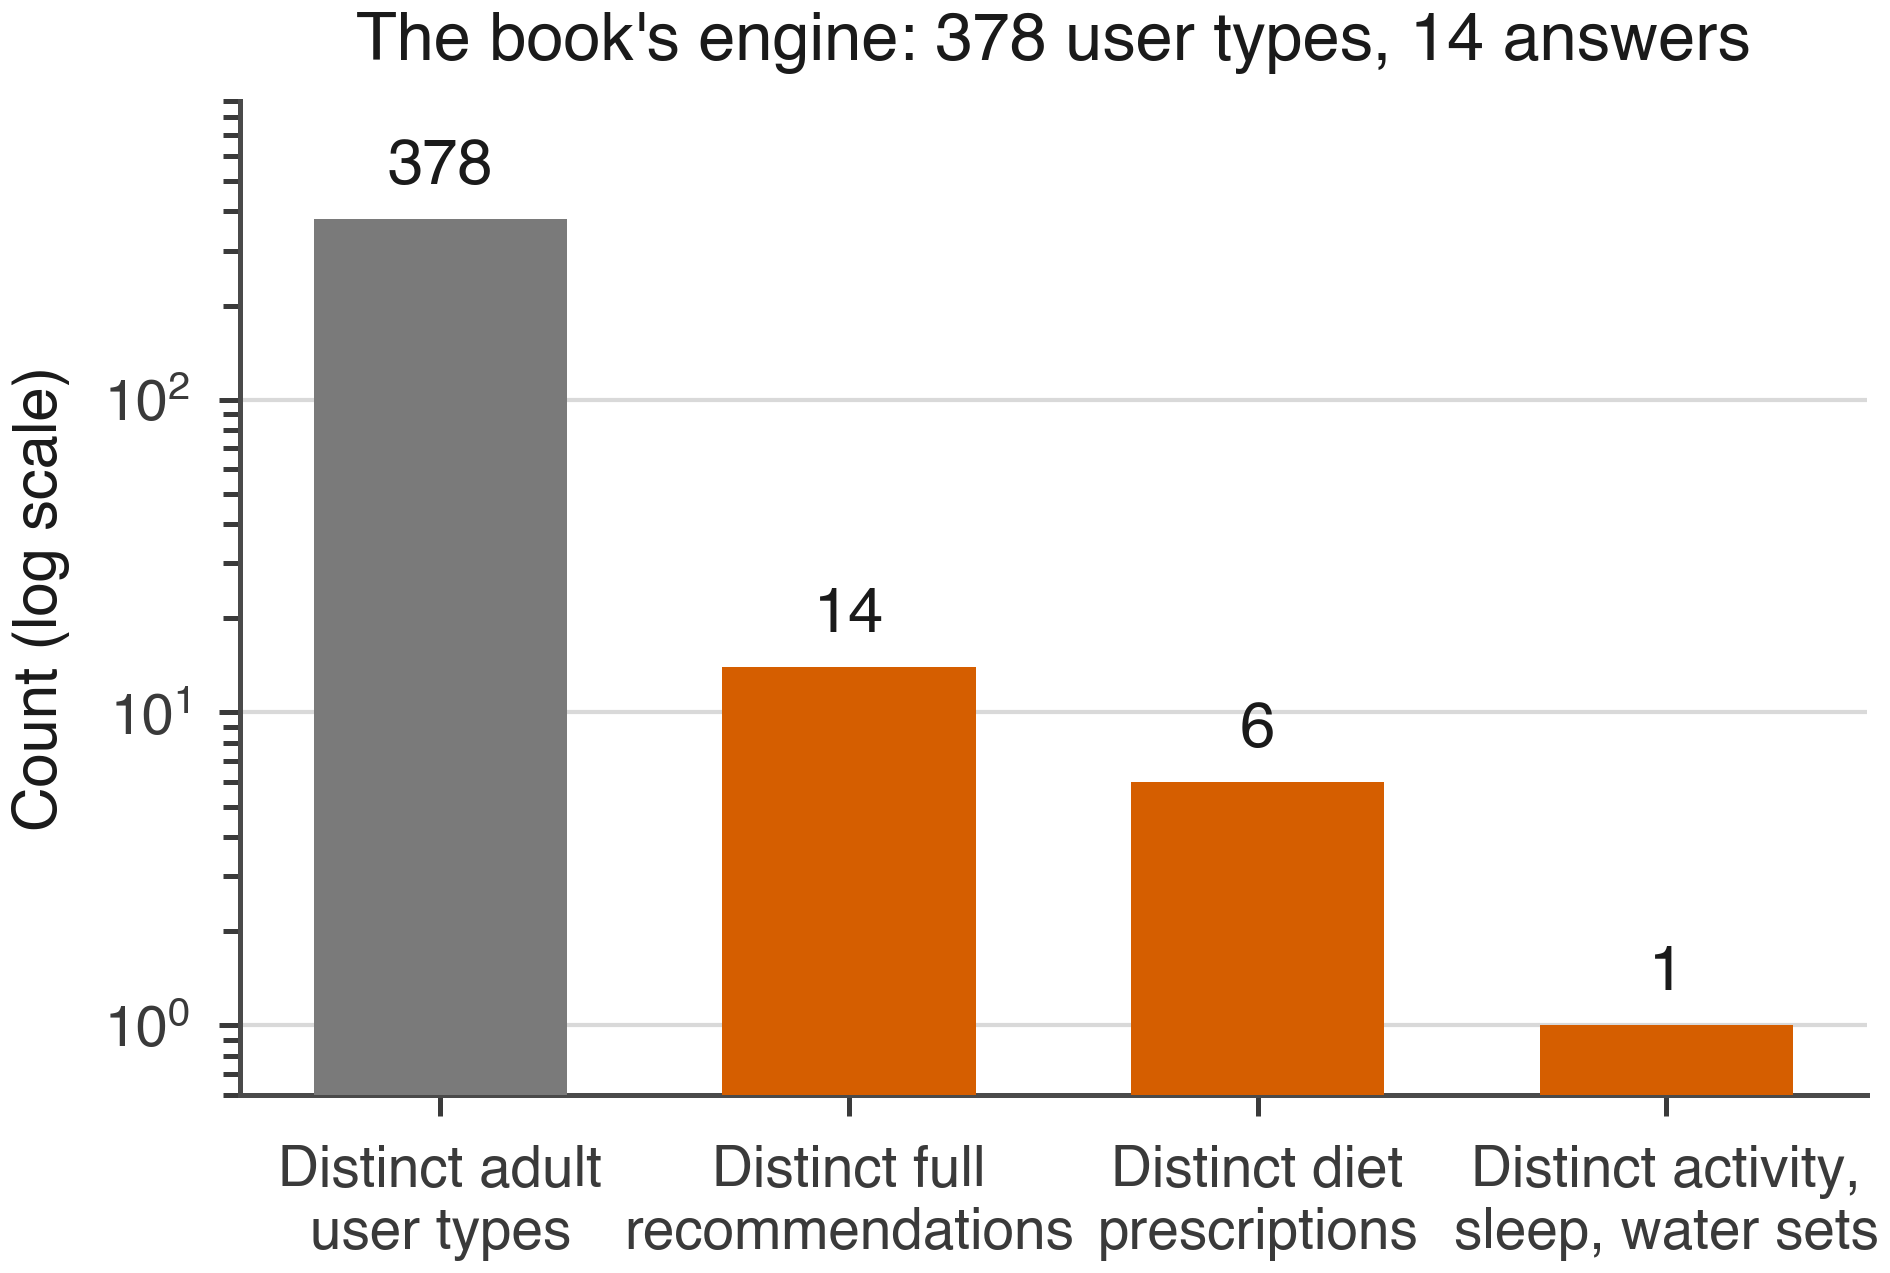
\includegraphics[width=\columnwidth]{f01_output_space.png}
\caption{The complete output space of the expert-authored engine. 378 distinct adult user types receive one of 14 distinct recommendations, and the activity, sleep, and fluid targets are a single constant across the entire grid.}
\label{fig:outputspace}
\end{figure}

The engine emits \textbf{14 distinct full recommendations}, comprising 6 distinct diet prescriptions and exactly \textbf{1} distinct activity, sleep, and fluid prescription. Its compression ratio, outputs divided by inputs, is 0.037. A calorie target is defined for only 19.0\% of the grid, because the book gives the 18 to 35 band and then states that the pattern continues without supplying the remaining values.

We stress the interpretation. This engine is faithful to WHO \cite{bull2020who}, Canadian \cite{ross2020canadian}, and US \cite{piercy2018pag} activity guidance and to ACSM prescription principles \cite{garber2011acsm}, and it is safe. Its serving targets follow an earlier edition of Canada's Food Guide; the 2019 revision removed per-demographic serving counts altogether \cite{healthcanada2019dietary}, which is the same conclusion this paper reaches by measurement. Its fluid target has no guideline source we could identify. It is also, structurally, a small lookup table, and it is a lookup table for a reason that has nothing to do with carelessness: population guidelines are written for populations. The rest of this paper measures what is missing.

%========================================
\section{Data and Screening}
\label{sec:battery}

\subsection{Screening}
Public datasets advertising fitness recommendations are frequently synthetic. Of 29 candidate datasets we acquired, 5 proved fabricated, and a single-column determination test of the kind used in data profiling \cite{huhtala1999tane, abedjan2015profiling} detects only one of them. We therefore screened every candidate with four complementary detectors before admitting it. The procedure, the evidence, and the per-dataset verdicts are given in the Appendix; only its outcome matters here, which is that the three sources below survived and the fabricated files were excluded.

\subsection{Datasets Used}
Three sources survive screening and carry what the ladder requires.

\textbf{NHANES 2013--2014} \cite{johnson2014nhanes} supplies L1 and L2 against behaviour in a nationally representative sample: 6{,}113 adults, 5{,}587 with a measured waist circumference, with survey design variables present; we follow the NCHS analytic guidelines \cite{nchs2018analytic}. Weekly moderate-equivalent activity is derived from the physical activity questionnaire with vigorous minutes doubled; median 150 minutes, with 33.1\% reporting none.

\textbf{LifeSnaps} \cite{yfantidou2022lifesnaps} is the backbone for L3 and L4: 71 adults wearing Fitbit devices, median 88 days each, with behaviour, sleep, heart rate, heart-rate variability, momentary self-report, and an explicit step goal.

\textbf{A second Fitbit cohort} \cite{furberg2016fitbit} (33 people, 31 days) provides independent replication. It carries no demographics at all, which is itself the situation an application is in on day one.

\subsection{Non-Wear}
Consumer wearables are accurate enough for step counting to support this analysis, with heart rate more variable \cite{fuller2020wearables, bai2018hr}. Non-wear is the dominant analysis hazard, and the convention differs by dataset; accelerometry practice defines explicit wear-time criteria for exactly this reason \cite{troiano2008, choi2011nonwear}, handling the resulting missing days is a studied problem in its own right \cite{lee2018missing}, and the number of days needed for a reliable individual estimate is an established question \cite{matthews2012best, tudorlocke2005days}. In LifeSnaps non-wear appears as a \textit{missing} step count, usually with exactly 1440 sedentary minutes: 2{,}633 of 7{,}410 person-days have missing steps, 2{,}256 of those record 1440 sedentary minutes, and only 86 days are literal zero-step days. In the second cohort the same condition appears as a literal \textit{zero}. Calories cannot disambiguate it, because the device emits basal metabolic rate on non-wear days. Treating either convention as real would manufacture sedentary behaviour that never happened. Filtering removes 36.5\% of person-days and retains 4{,}704 days across all 71 people.

%========================================
\section{What Static Profiles Explain}

\subsection{Method}
On NHANES we fit weighted least squares with examination weights and compute confidence intervals by a delete-one-PSU jackknife over the 15 strata by 2 PSU design. We predict two families of target on the same people: \textit{body} (waist circumference, waist-to-height ratio) and \textit{behaviour} (weekly activity, sedentary minutes, sleep hours). Predictor sets containing a component of the target are excluded as circular.

\subsection{Result}
Fig.~\ref{fig:nhanes} gives the comparison. Age and sex explain 7.9\% of the variance in waist-to-height ratio; adding BMI raises this to 89.5\%. The same ladder applied to weekly activity moves from 7.4\% to 7.4\%. Adding waist gives 7.5\%.

\begin{figure}[t]
\centering
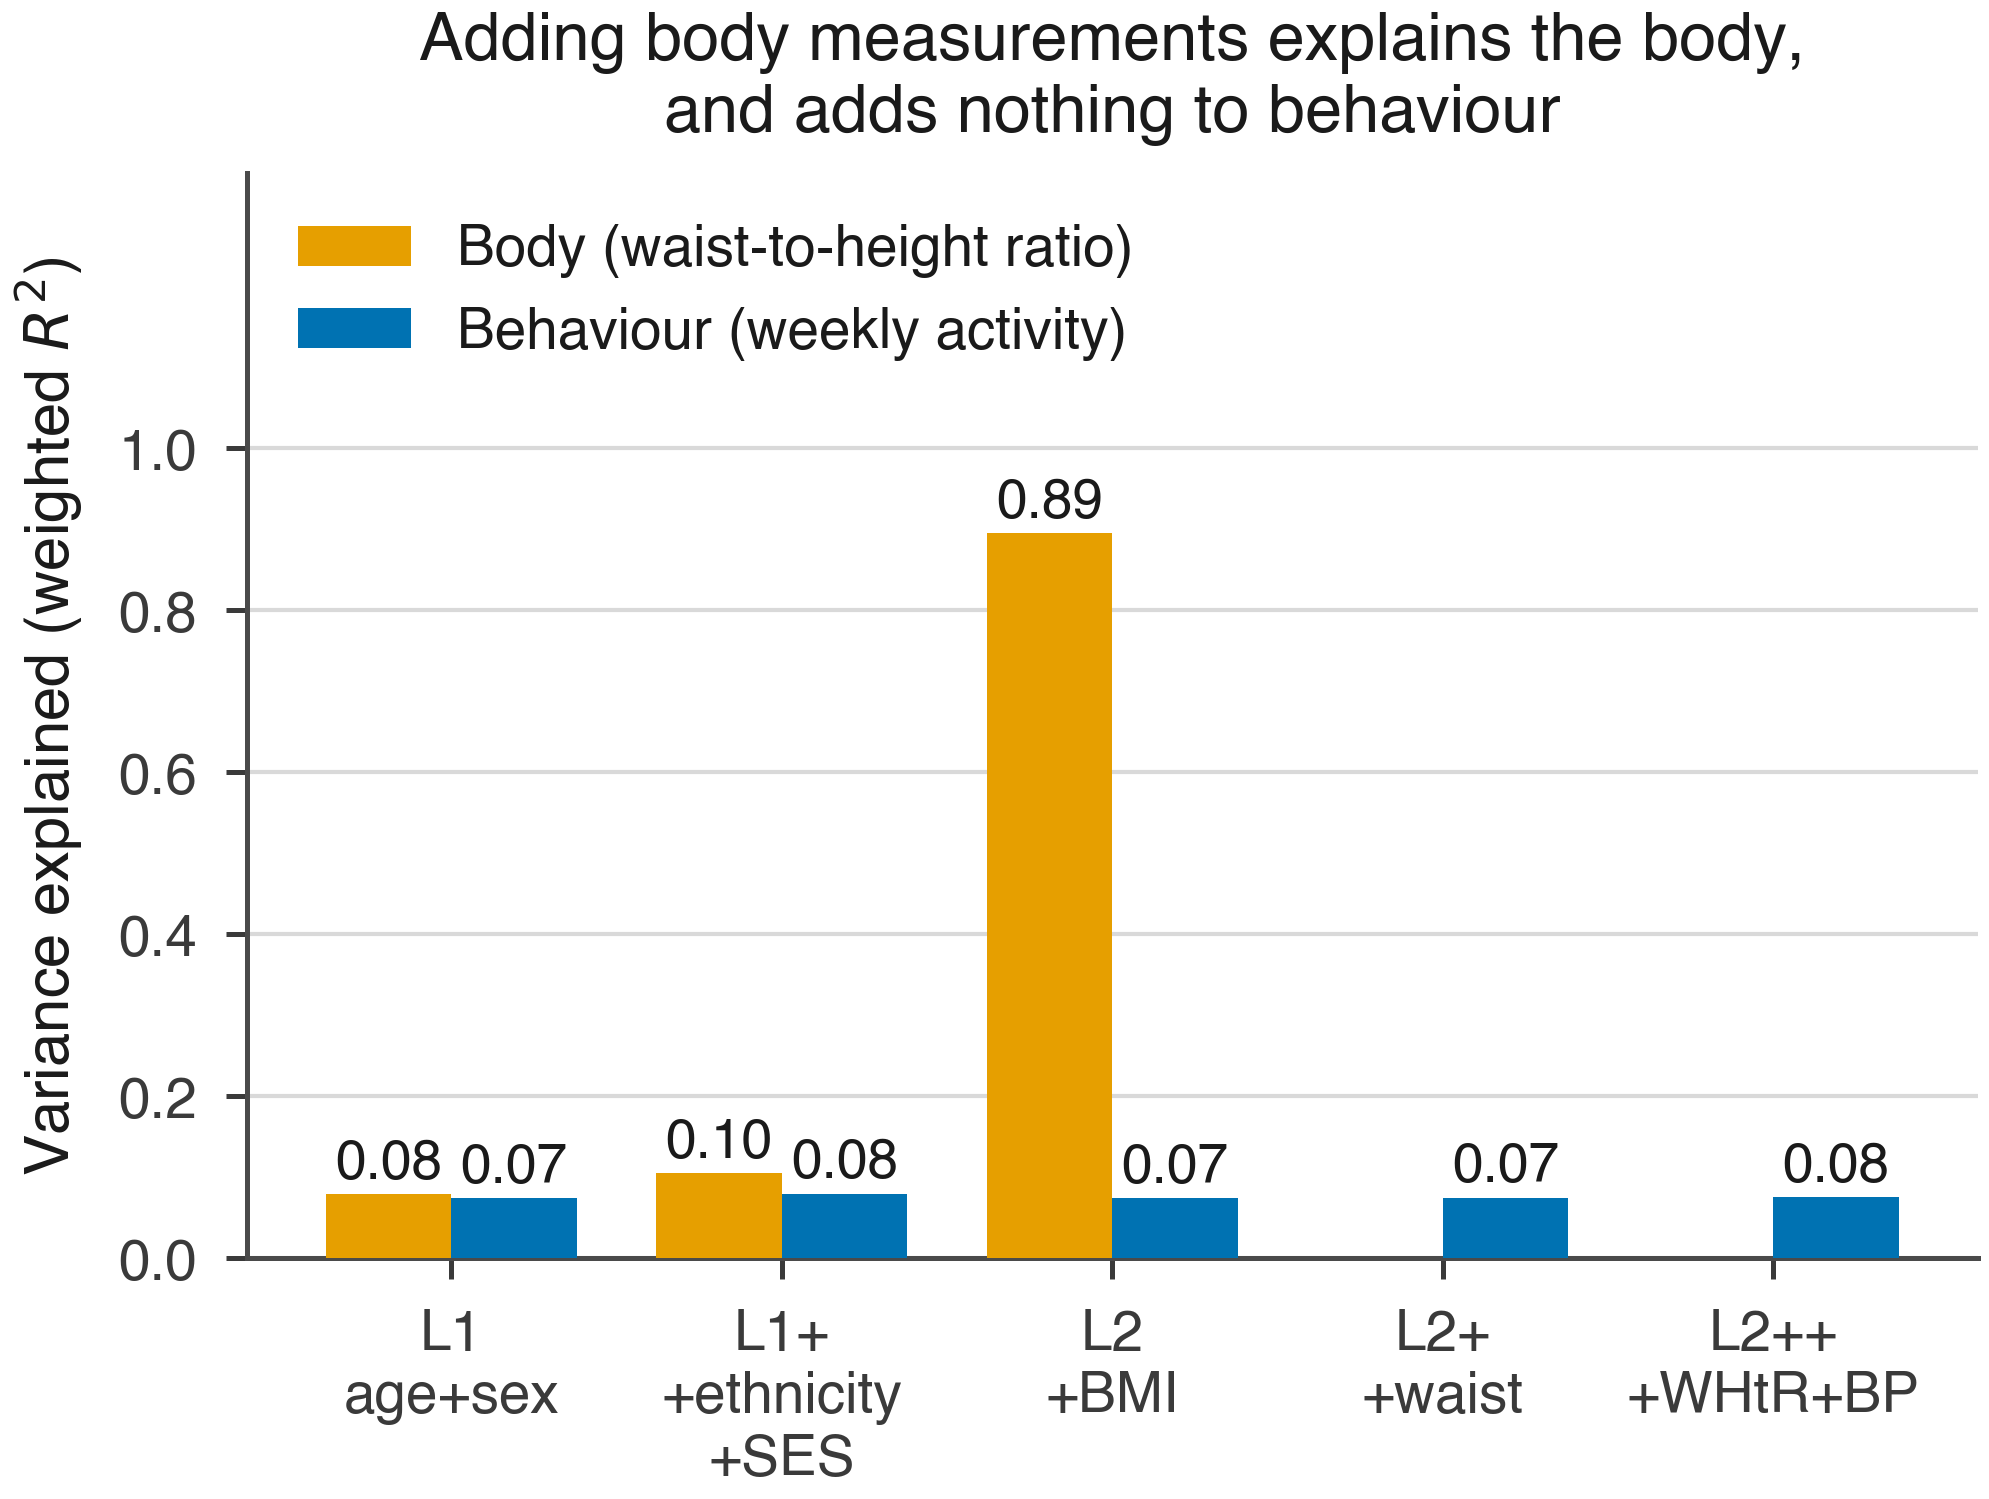
\includegraphics[width=\columnwidth]{f04_nhanes_body_vs_behaviour.png}
\caption{NHANES 2013--2014, design-weighted. Adding body measurements to age and sex explains the body more than tenfold better and adds nothing to behaviour.}
\label{fig:nhanes}
\end{figure}

For predicting who meets the activity guideline, age and sex give AUC 0.6686; adding BMI gives 0.6686; adding waist gives 0.6637, which is slightly worse. As single predictors, waist-to-height ratio (0.5868) beats BMI (0.5366), reproducing the established ordering, but age alone (0.6497) beats both.

Climbing from L1 to L2, the most natural improvement available to a developer, buys nothing at all for behaviour.

%========================================
\section{Why: Bodies Are Stable, Behaviour Is Not}

If behaviour were a stable personal trait, some profile would predict it. We test that directly with a one-way random-effects intraclass correlation on LifeSnaps, with a cluster bootstrap over people (Fig.~\ref{fig:icc}).

\begin{figure}[t]
\centering
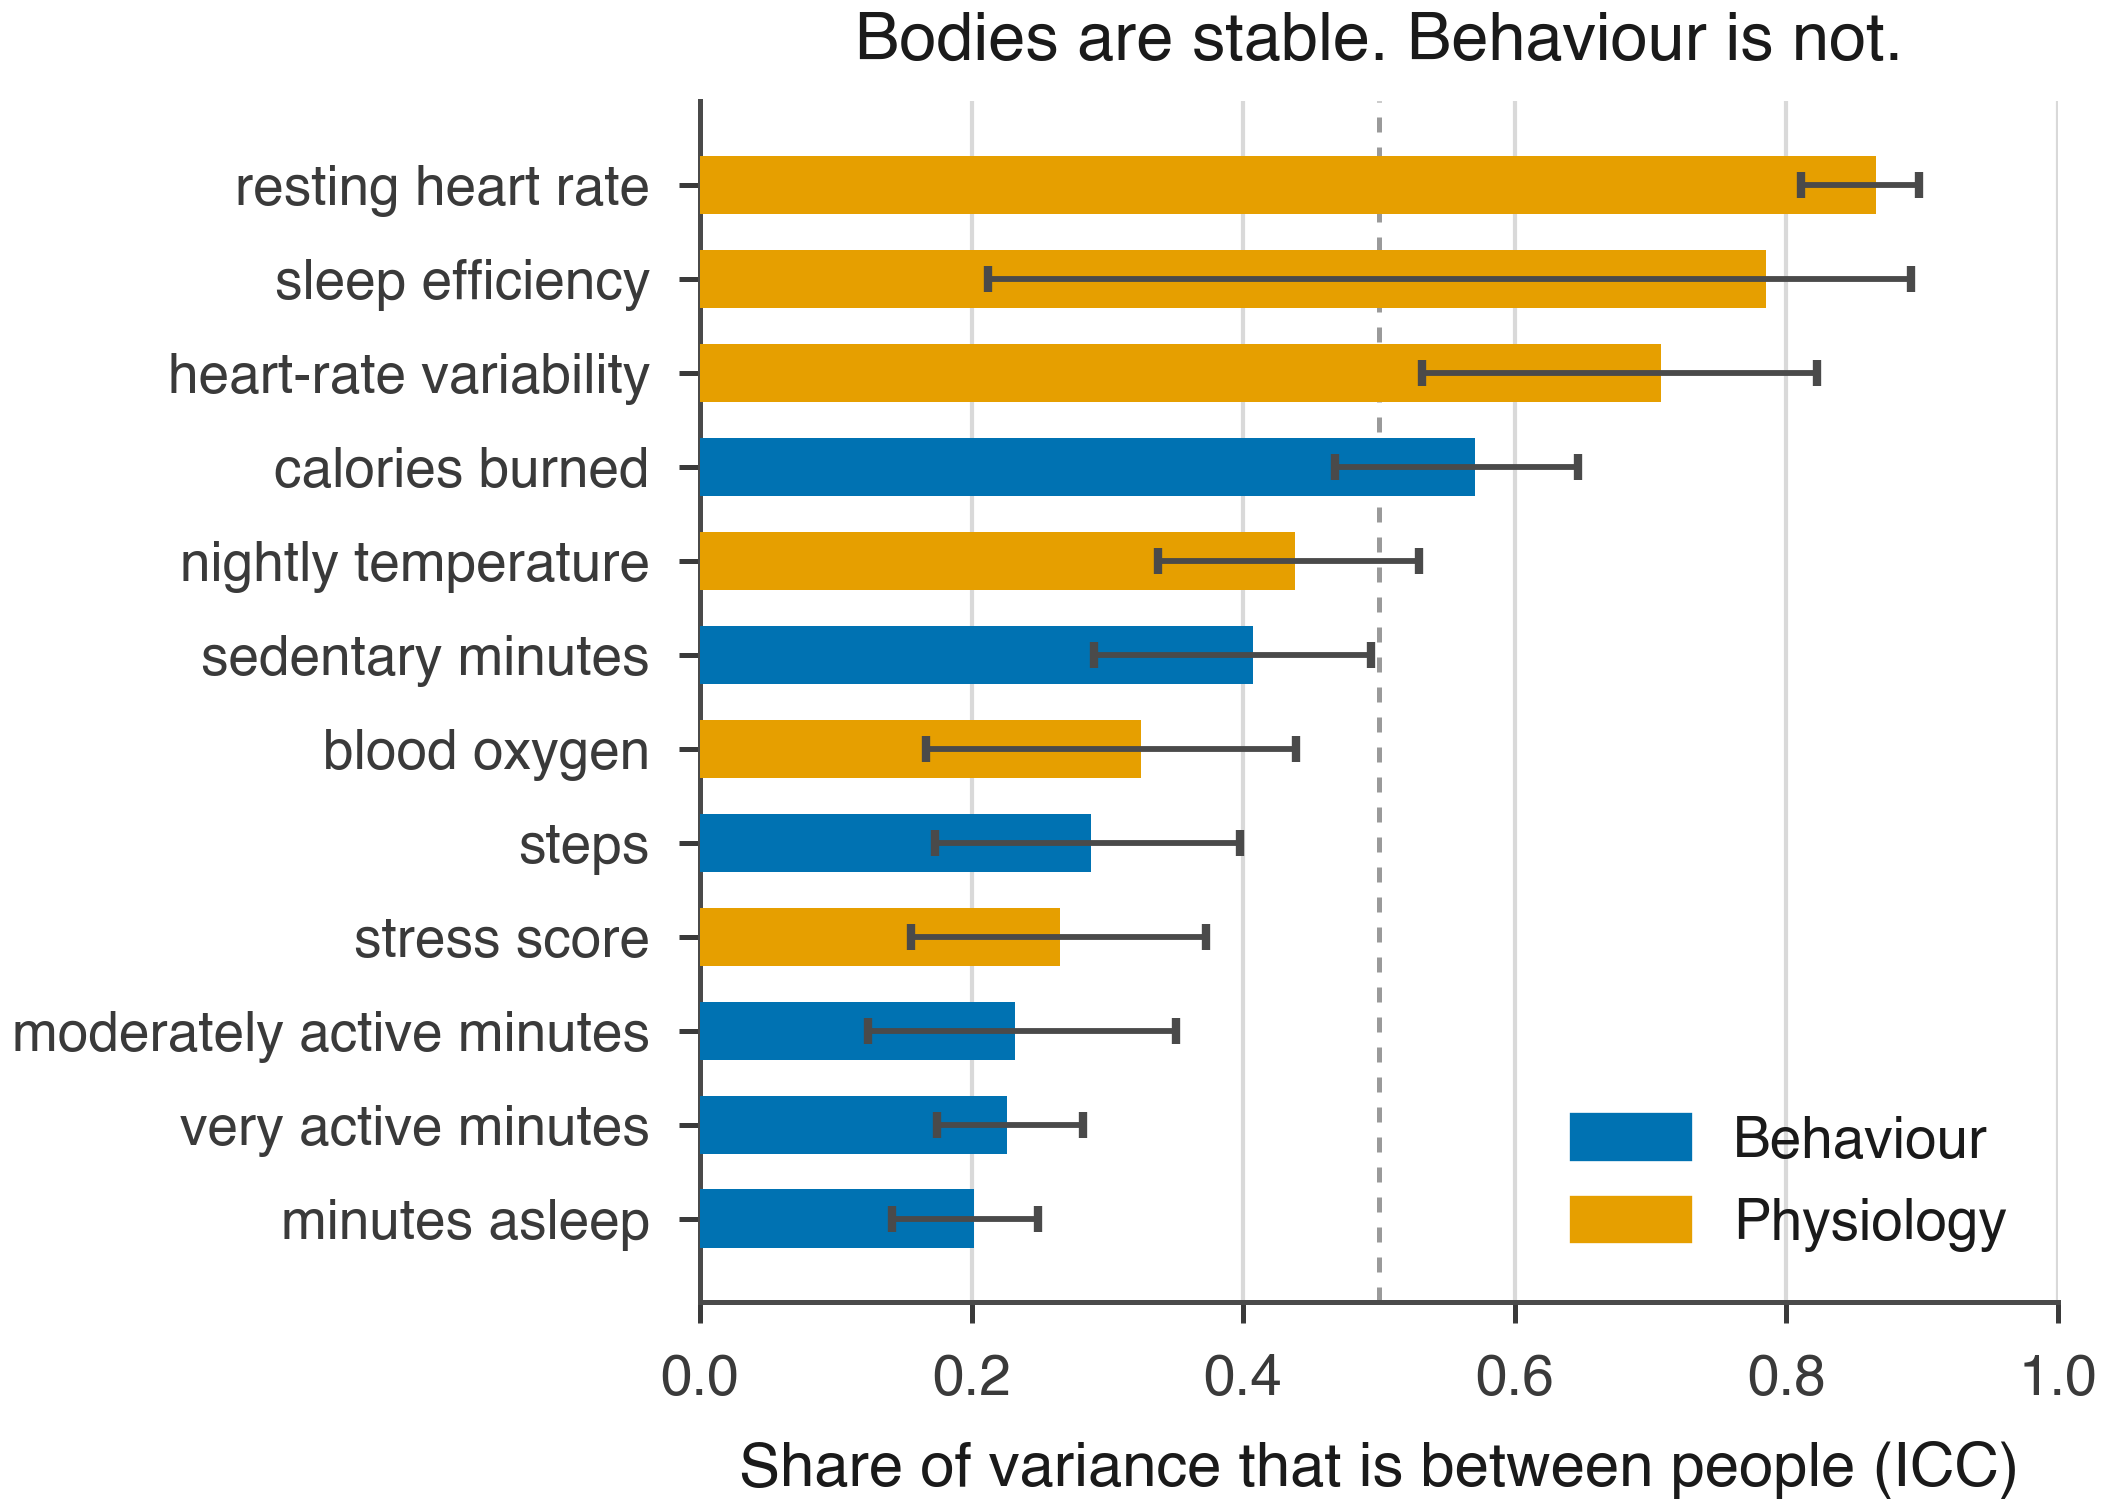
\includegraphics[width=\columnwidth]{f05_icc.png}
\caption{Share of variance that lies between people rather than within them. Resting heart rate is 87\% a property of the person; step count is 29\% a property of the person and 71\% a property of the day.}
\label{fig:icc}
\end{figure}

The median ICC is \textbf{0.26 for behaviour} and \textbf{0.57 for physiology}. Resting heart rate reaches 0.866 and sleep efficiency 0.785, while step count is 0.288 and very active minutes 0.226.

This is a ceiling result. A static profile, however rich, can account for at most the between-person share. For behaviour that is roughly a quarter. The remaining three quarters is which day it happens to be, and no onboarding form of any length can reach it. It also explains the previous section rather than merely accompanying it: static profiles predict the body well because the body is a trait, and predict behaviour badly because behaviour largely is not.

%========================================
\section{The Ladder, Measured}

\subsection{Protocol}
We predict next-day step count and next-day very active minutes. Every history feature is shifted so that day $t$ is predicted only from days strictly before $t$, and every rolling statistic is computed on an expanding window of that person's own past. Evaluation is forward-chained over the pooled calendar, so every fold trains on the past and tests on the future, following rolling-origin practice for temporally ordered data \cite{tashman2000oos}. We note that $k$-fold cross-validation can be valid for purely autoregressive models with uncorrelated errors \cite{bergmeir2018arcv}, and that blocked designs are often preferable to reserving only the end of a series \cite{bergmeir2012tscv}; forward chaining is the conservative choice here and is what a deployed system actually faces. We are explicit about which generalization this tests. The folds are temporal, not person-held-out, so the same participants appear in training and test at different times. That is deliberate: it is the deployment case in which an application already knows a user and must forecast their future. It is therefore NOT a test of generalization to a new person, and we do not report it as one. Section~\ref{sec:coldstart} runs the complementary leave-one-person-out design, in which the model has never seen the test participant, and finds a slightly higher L3 value ($+0.2749$), so the ordering reported here is not an artefact of participant overlap. Record-wise splits that mix a person's days at random would leak identity and inflate accuracy \cite{saeb2017usecase, roberts2017blockcv}; forward chaining avoids that by construction because no test day precedes any training day. The trade-offs are surveyed in \cite{arlot2010cvsurvey, little2017cvperspectives}. We report ridge as the headline and gradient boosting alongside: if the ordering of rungs is the same under both, the conclusion concerns the available information rather than the model.

\subsection{Result}

\begin{figure}[t]
\centering
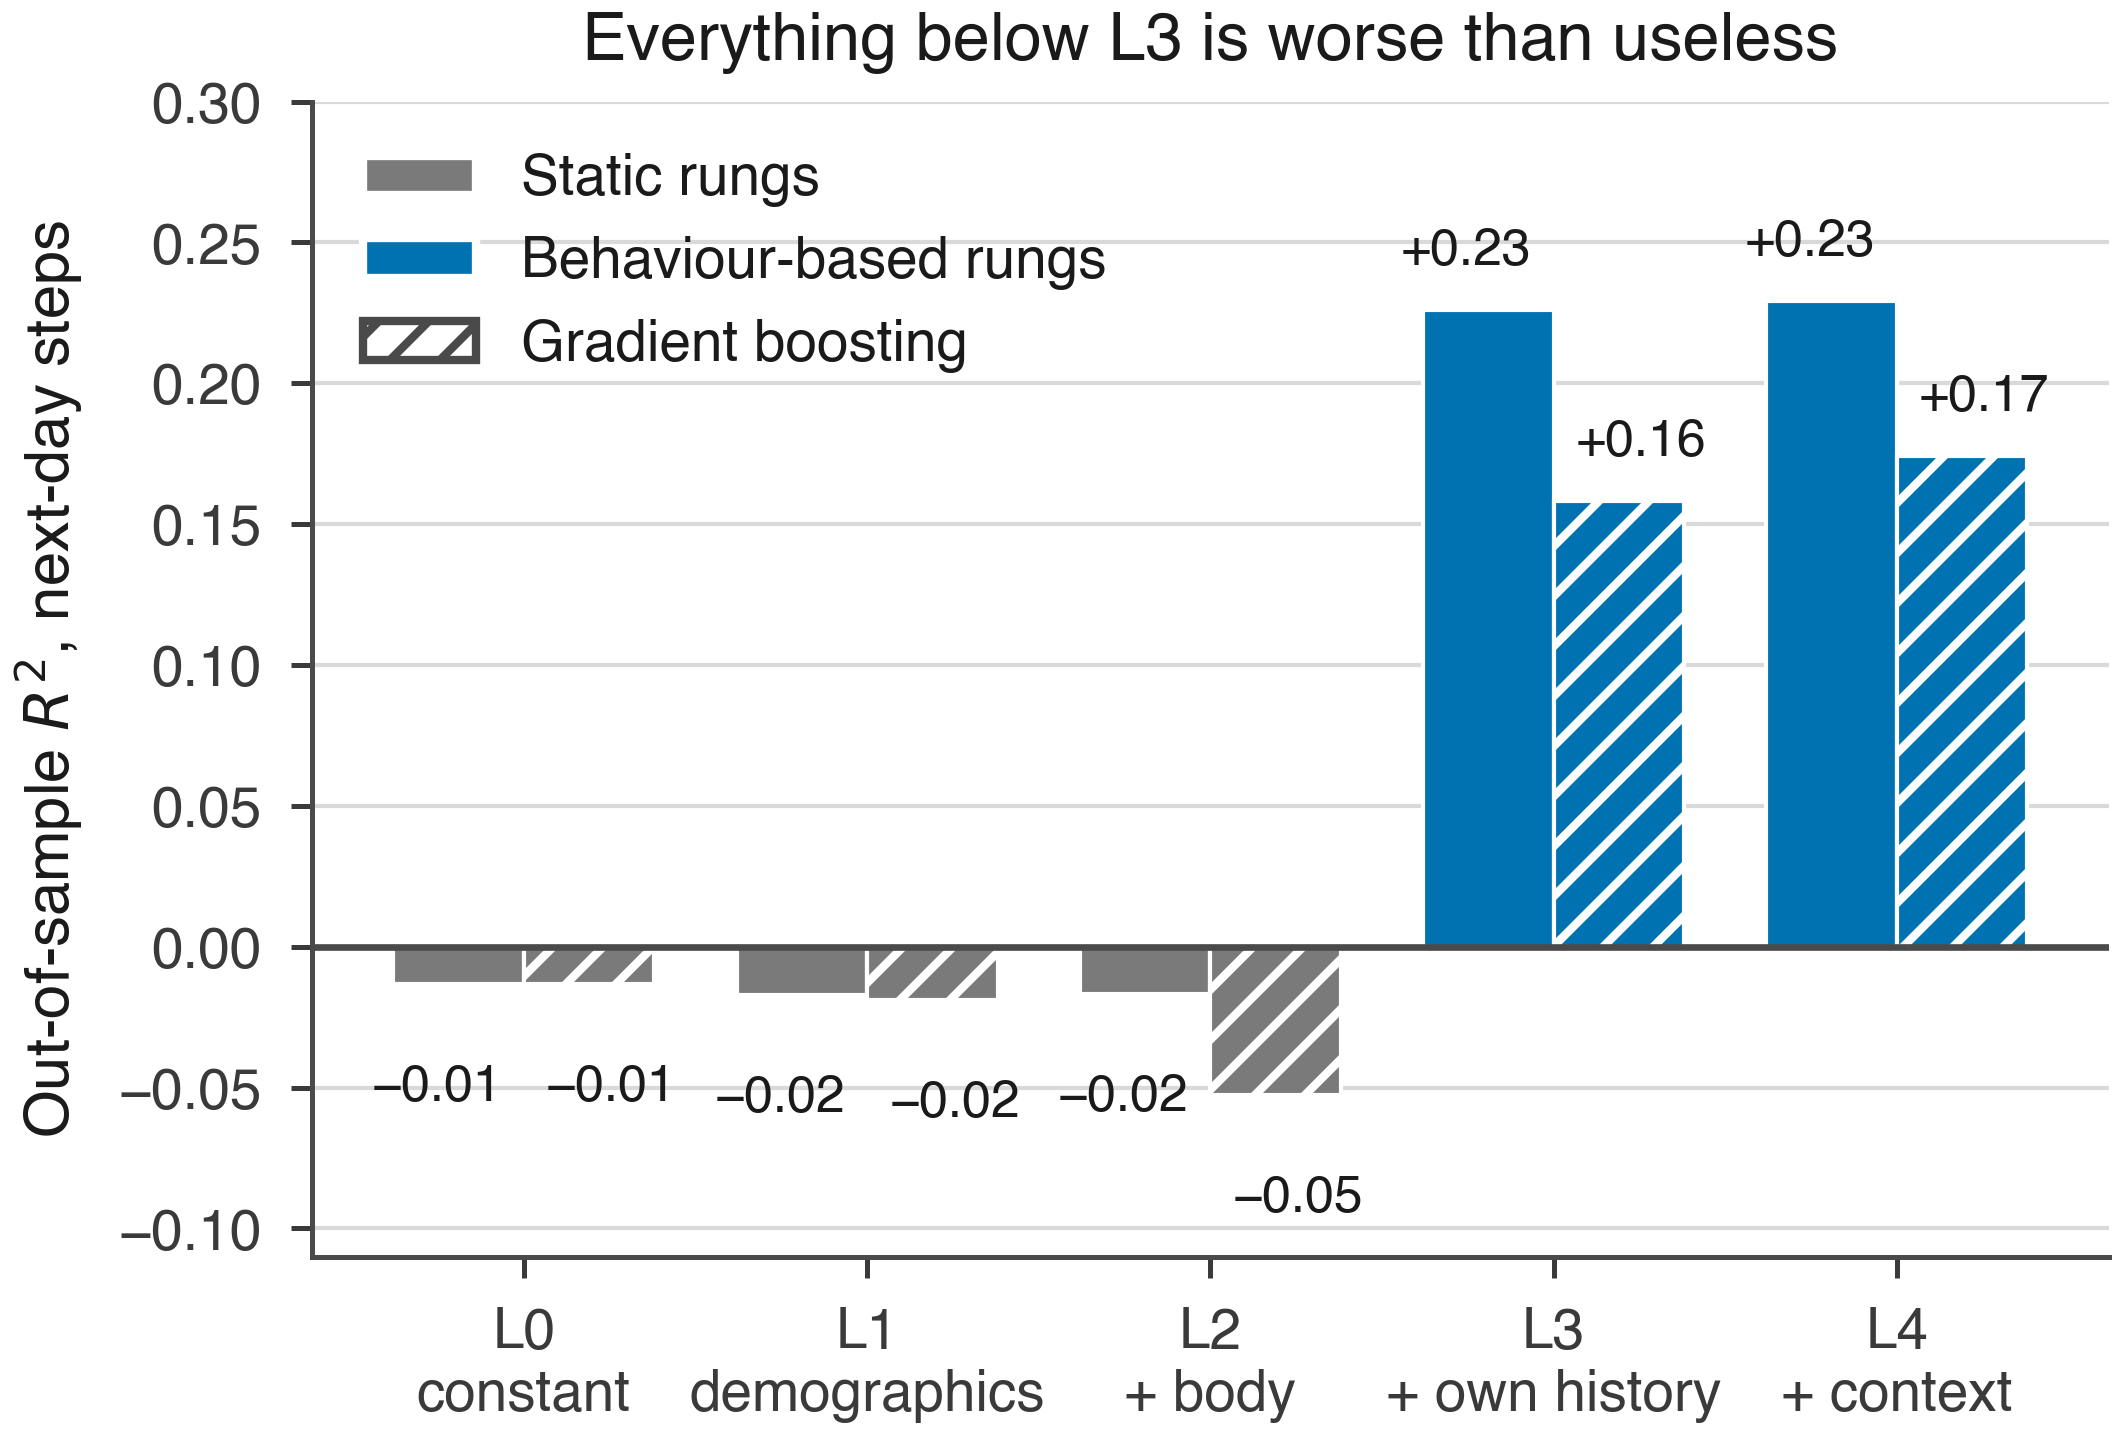
\includegraphics[width=\columnwidth]{f06_ladder.png}
\caption{Out-of-sample $R^2$ for next-day step count on LifeSnaps. The three static rungs are all negative: predicting the population average is worse than doing nothing. The gain arrives entirely at L3.}
\label{fig:ladder}
\end{figure}

\begin{table}[t]
\centering
\caption{The Ladder on Next-Day Step Count (LifeSnaps, Ridge, Forward-Chained). Marginal Gains Are Paired Cluster-Bootstrap Estimates Over 300 Resamples of Participants}
\begin{tabular}{@{}lrrl@{}}
\toprule
\textbf{Rung} & \textbf{$R^2$} & \textbf{MAE} & \textbf{Marginal gain [95\% CI]} \\
\midrule
L0 population constant     & $-0.0131$ & 4{,}122 & \\
L1 demographics (the book) & $-0.0173$ & 4{,}133 & $-0.0038$ [$-0.071$, $+0.032$] \\
L2 + body measurements     & $-0.0168$ & 4{,}133 & $+0.0001$ [$-0.055$, $+0.022$] \\
L3 + own behaviour history & $+0.2261$ & 3{,}457 & $\mathbf{+0.2432}$ [$+0.143$, $+0.369$] \\
L4 + yesterday's context   & $+0.2292$ & 3{,}454 & $+0.0029$ [$-0.013$, $+0.009$] \\
\bottomrule
\end{tabular}
\label{tab:ladder}
\end{table}

Table~\ref{tab:ladder} and Fig.~\ref{fig:ladder} give the result. Intervals come from a cluster bootstrap over participants, resampling people rather than days, with each marginal gain bootstrapped paired within a replicate. Only one step on the ladder is distinguishable from zero: the move to L3, at $+0.243$ with a 95\% interval of $[+0.143, +0.369]$. Neither the L1-to-L2 step nor the L3-to-L4 step separates from zero, so the correct reading of those is that they buy nothing measurable, not that they actively hurt. For next-day step count, L0, L1, and L2 all have negative $R^2$. This does not hold universally: for very active minutes (Fig.~\ref{fig:replication}) L1 and L2 are marginally positive at $+0.016$ and $+0.018$, still an order of magnitude below L3. The robust statement is that the static rungs sit at or below zero, not that they are always negative. Out of sample the coefficient of determination is unbounded below, and a negative value means the model predicts the held-out data worse than a horizontal line through its mean \cite{chicco2021r2, alexander2015bewarer2, poldrack2020prediction}. L3 reaches $+0.2261$ and reduces mean absolute error by 665 steps per day. L4 adds $+0.0032$.

Fig.~\ref{fig:features} shows which features carry the L3 gain. The person's own long-run average and their recent trend dominate; age, sex, and BMI sit near zero even when the model is free to use them.

\begin{figure}[t]
\centering
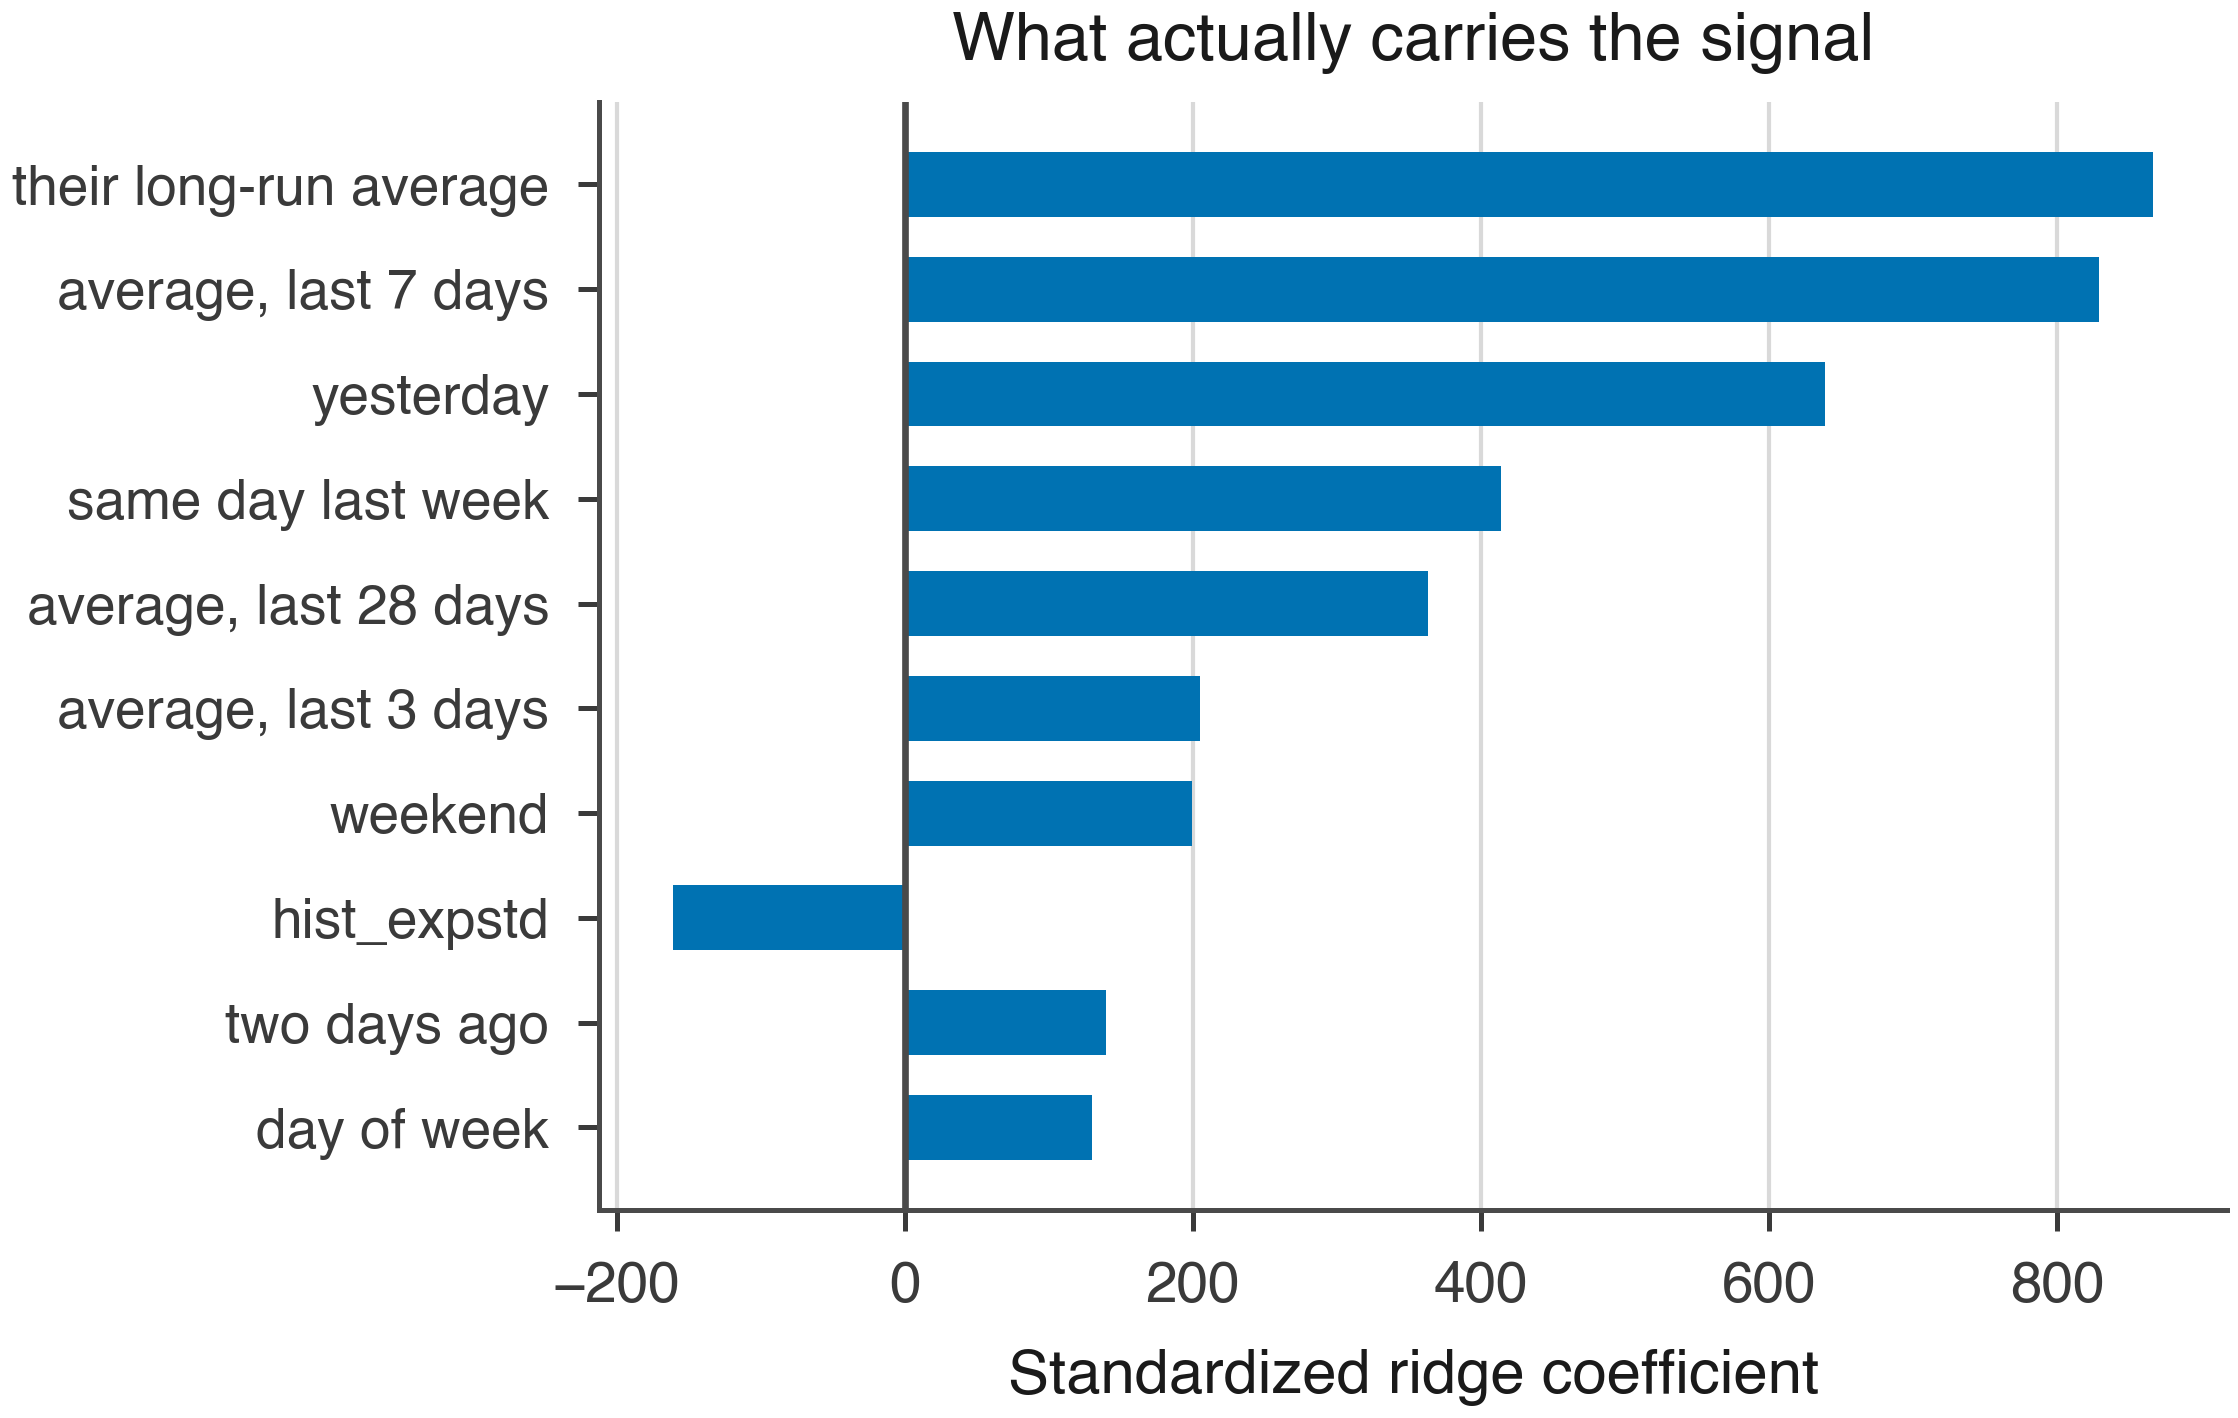
\includegraphics[width=\columnwidth]{f11_feature_importance.png}
\caption{Standardized ridge coefficients for the L3 feature set. What predicts tomorrow is the person's own recent behaviour, not any description of their body.}
\label{fig:features}
\end{figure}

Fig.~\ref{fig:replication} shows the same ordering for a second outcome and in an independent cohort, under both model families. In the second cohort, which has no demographics at all, L0 gives $-0.0040$ and L3 gives $+0.3396$.

\begin{figure*}[t]
\centering
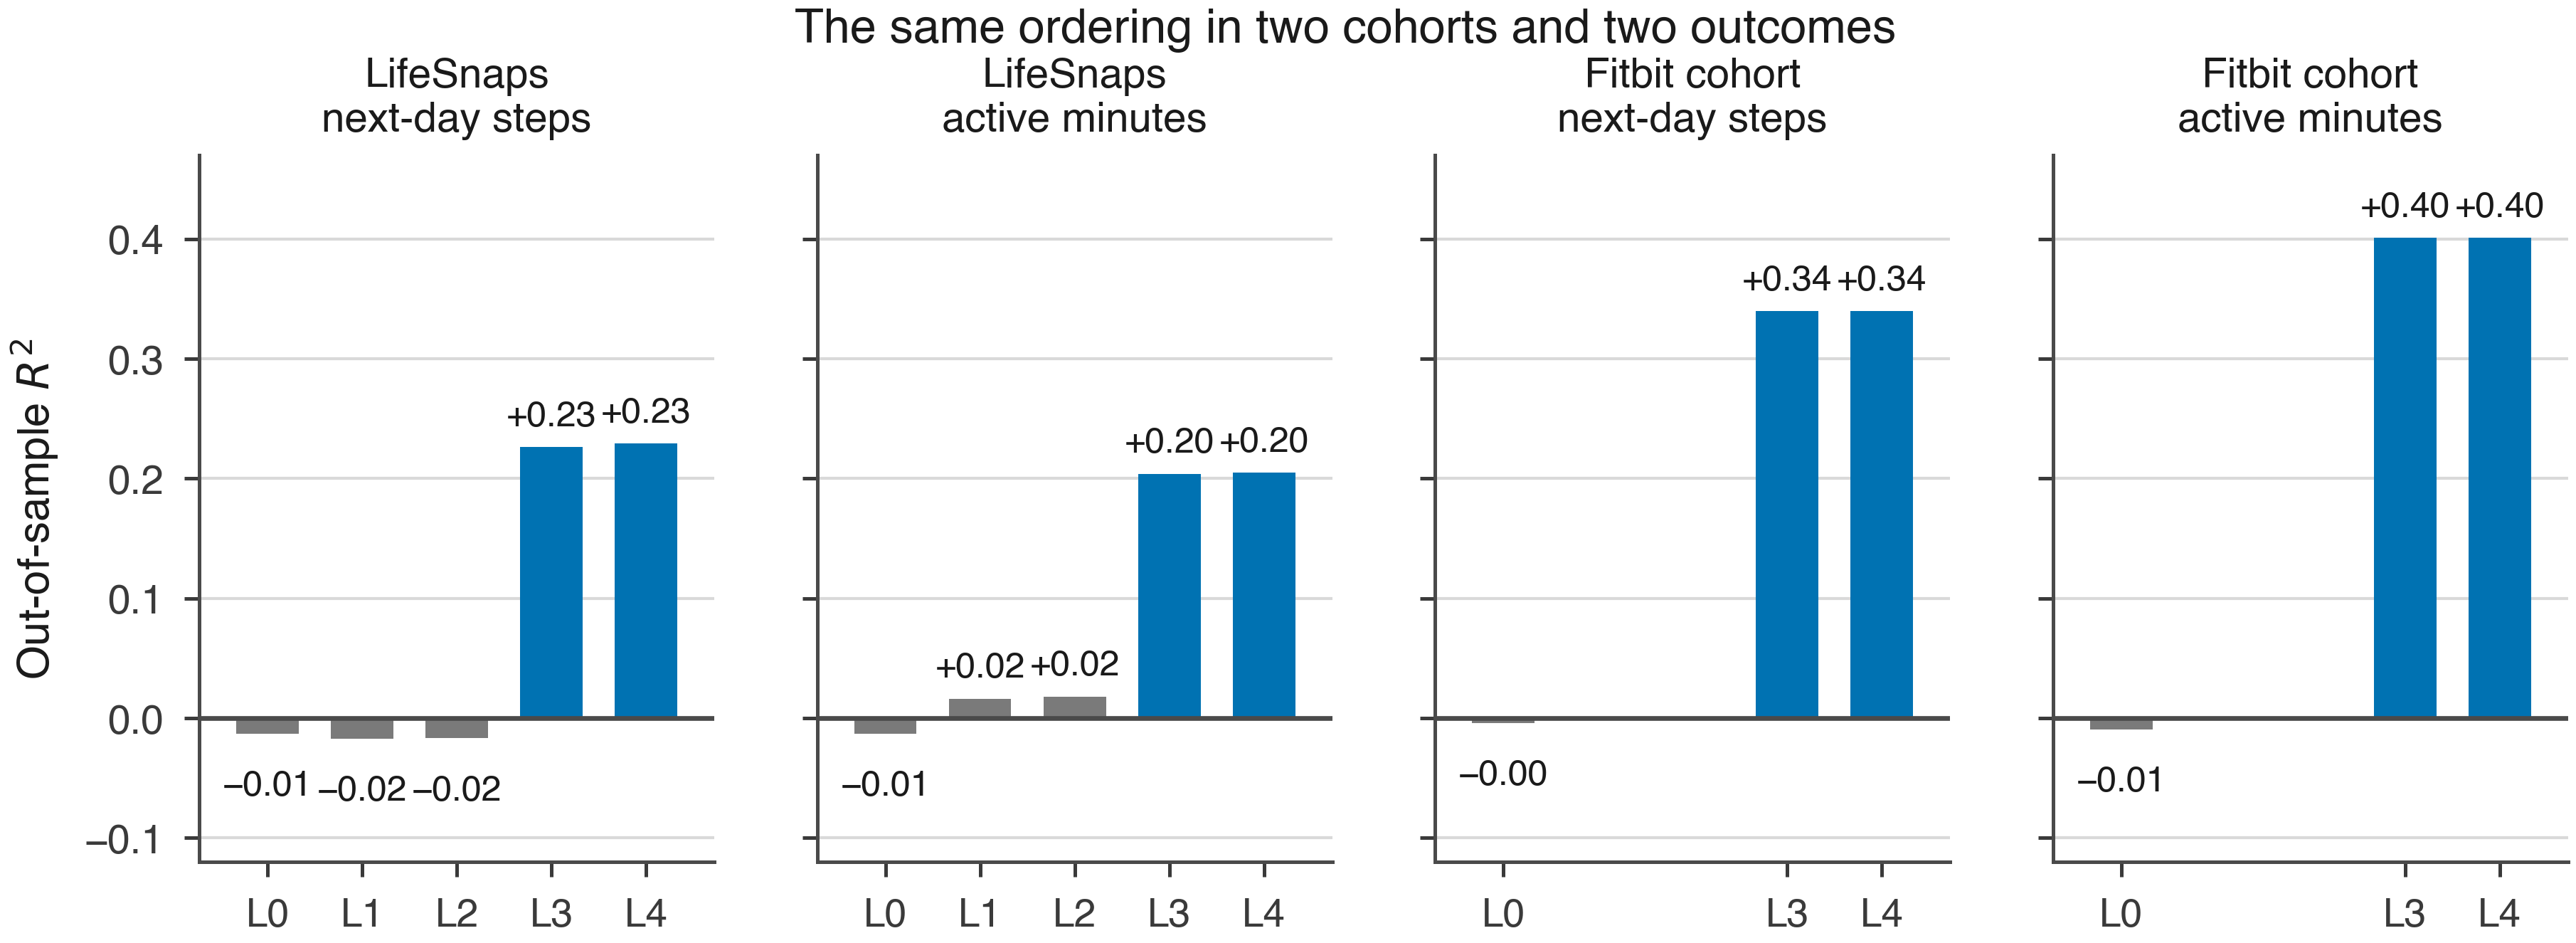
\includegraphics[width=\textwidth]{f07_ladder_replication.png}
\caption{The ordering replicates across two cohorts and two outcomes. The second cohort carries no demographic variables, so only L0, L3, and L4 are defined there.}
\label{fig:replication}
\end{figure*}

%========================================
\section{Adherence}
\label{sec:adherence}

Predicting what somebody will do is not the same as predicting whether they will do what is suggested. LifeSnaps records a real step goal, so goal attainment is an observed adherence outcome rather than a constructed one. We note a limitation: the goal is stored binned, as a labelled range, so the exact target each participant set is not recoverable. We use the lower bound of the band, which understates strictness; this raises the measured base rate and is declared rather than hidden.

The quantity a recommender needs is not the benefit of an action but the benefit weighted by the probability it is performed. Fig.~\ref{fig:adherence} estimates that probability.

\begin{figure}[t]
\centering
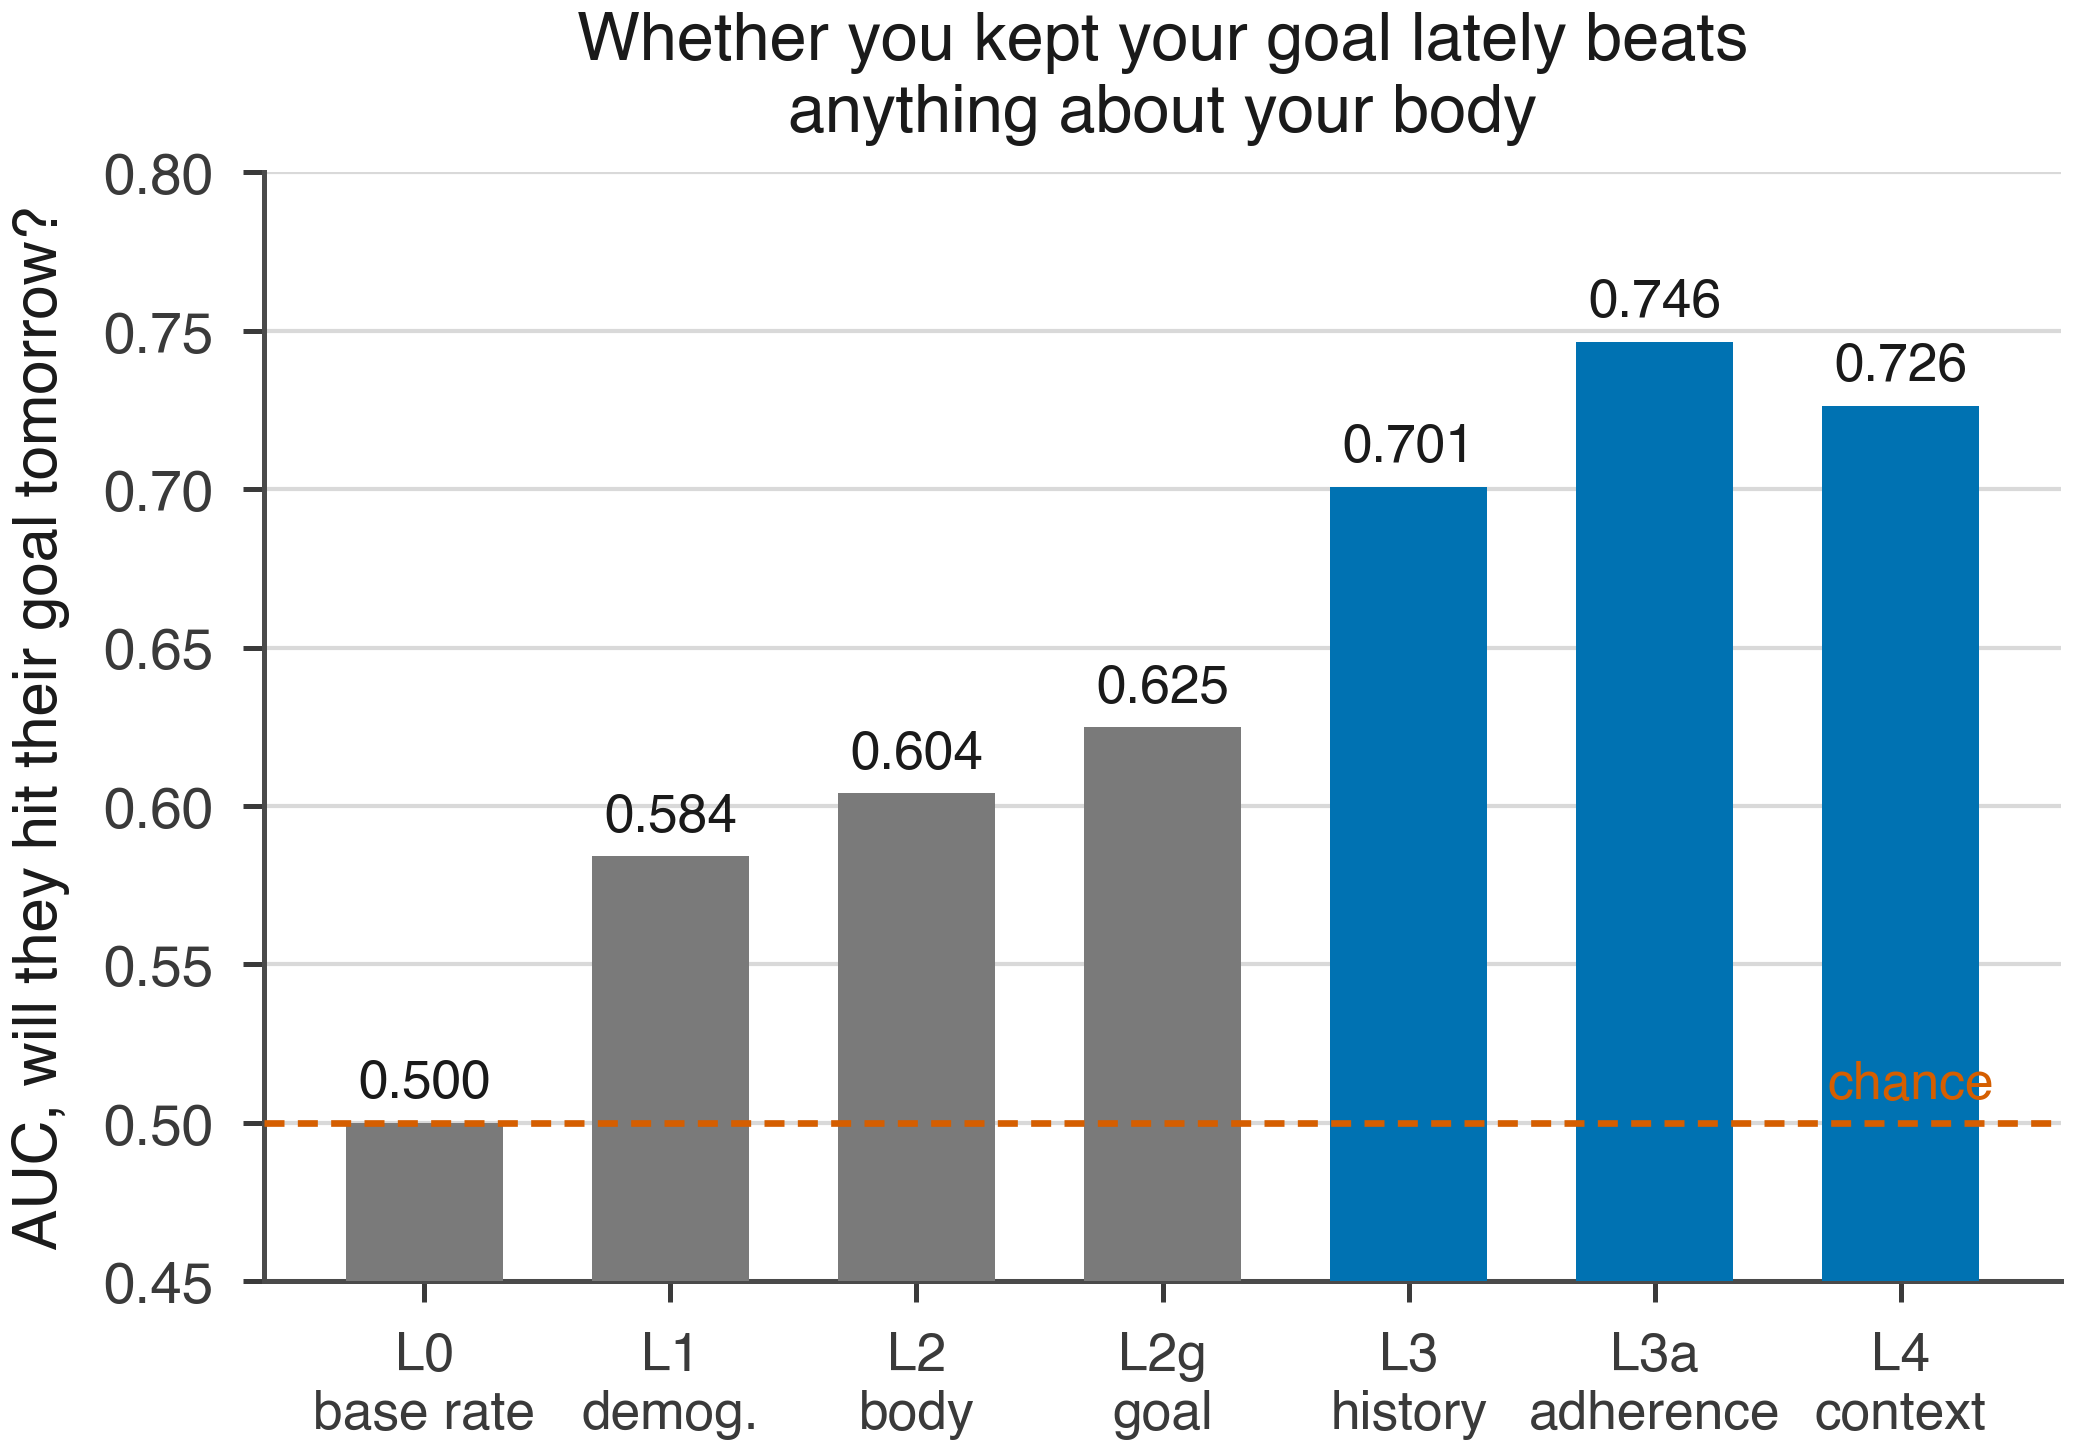
\includegraphics[width=\columnwidth]{f08_adherence.png}
\caption{Predicting whether a person meets their step goal tomorrow. A static description of the person reaches AUC 0.604; their own recent adherence reaches 0.746.}
\label{fig:adherence}
\end{figure}

A static profile reaches AUC 0.604 (Brier 0.1554). Adding the person's own behaviour history gives 0.701, and adding their own recent adherence gives \textbf{0.746} (Brier 0.1376). Adding continuous context reduces performance to 0.726.

We must be careful about what this supports. With 51 participants, of whom 39 have a varying outcome, the cluster bootstrap gives wide intervals: L2 is 0.604 $[0.392, 0.695]$ and L3a is 0.746 $[0.617, 0.794]$, and \emph{no adjacent pair separates from zero}. What the data do support is that the full behaviour-and-adherence model is better than chance, since its interval excludes 0.5 by a wide margin, while the static profile's does not. The ordering is consistent with the step-count result and with the variance decomposition, but on this sample it is suggestive rather than established, and we report it that way.

%========================================
\section{Cold Start}
\label{sec:coldstart}

L3 requires history that a new user does not have. We evaluate leave-one-person-out, so the model has never seen the test person, and bucket every prediction by how many days of that person's own history existed when it was made (Fig.~\ref{fig:coldstart}).

\begin{figure}[t]
\centering
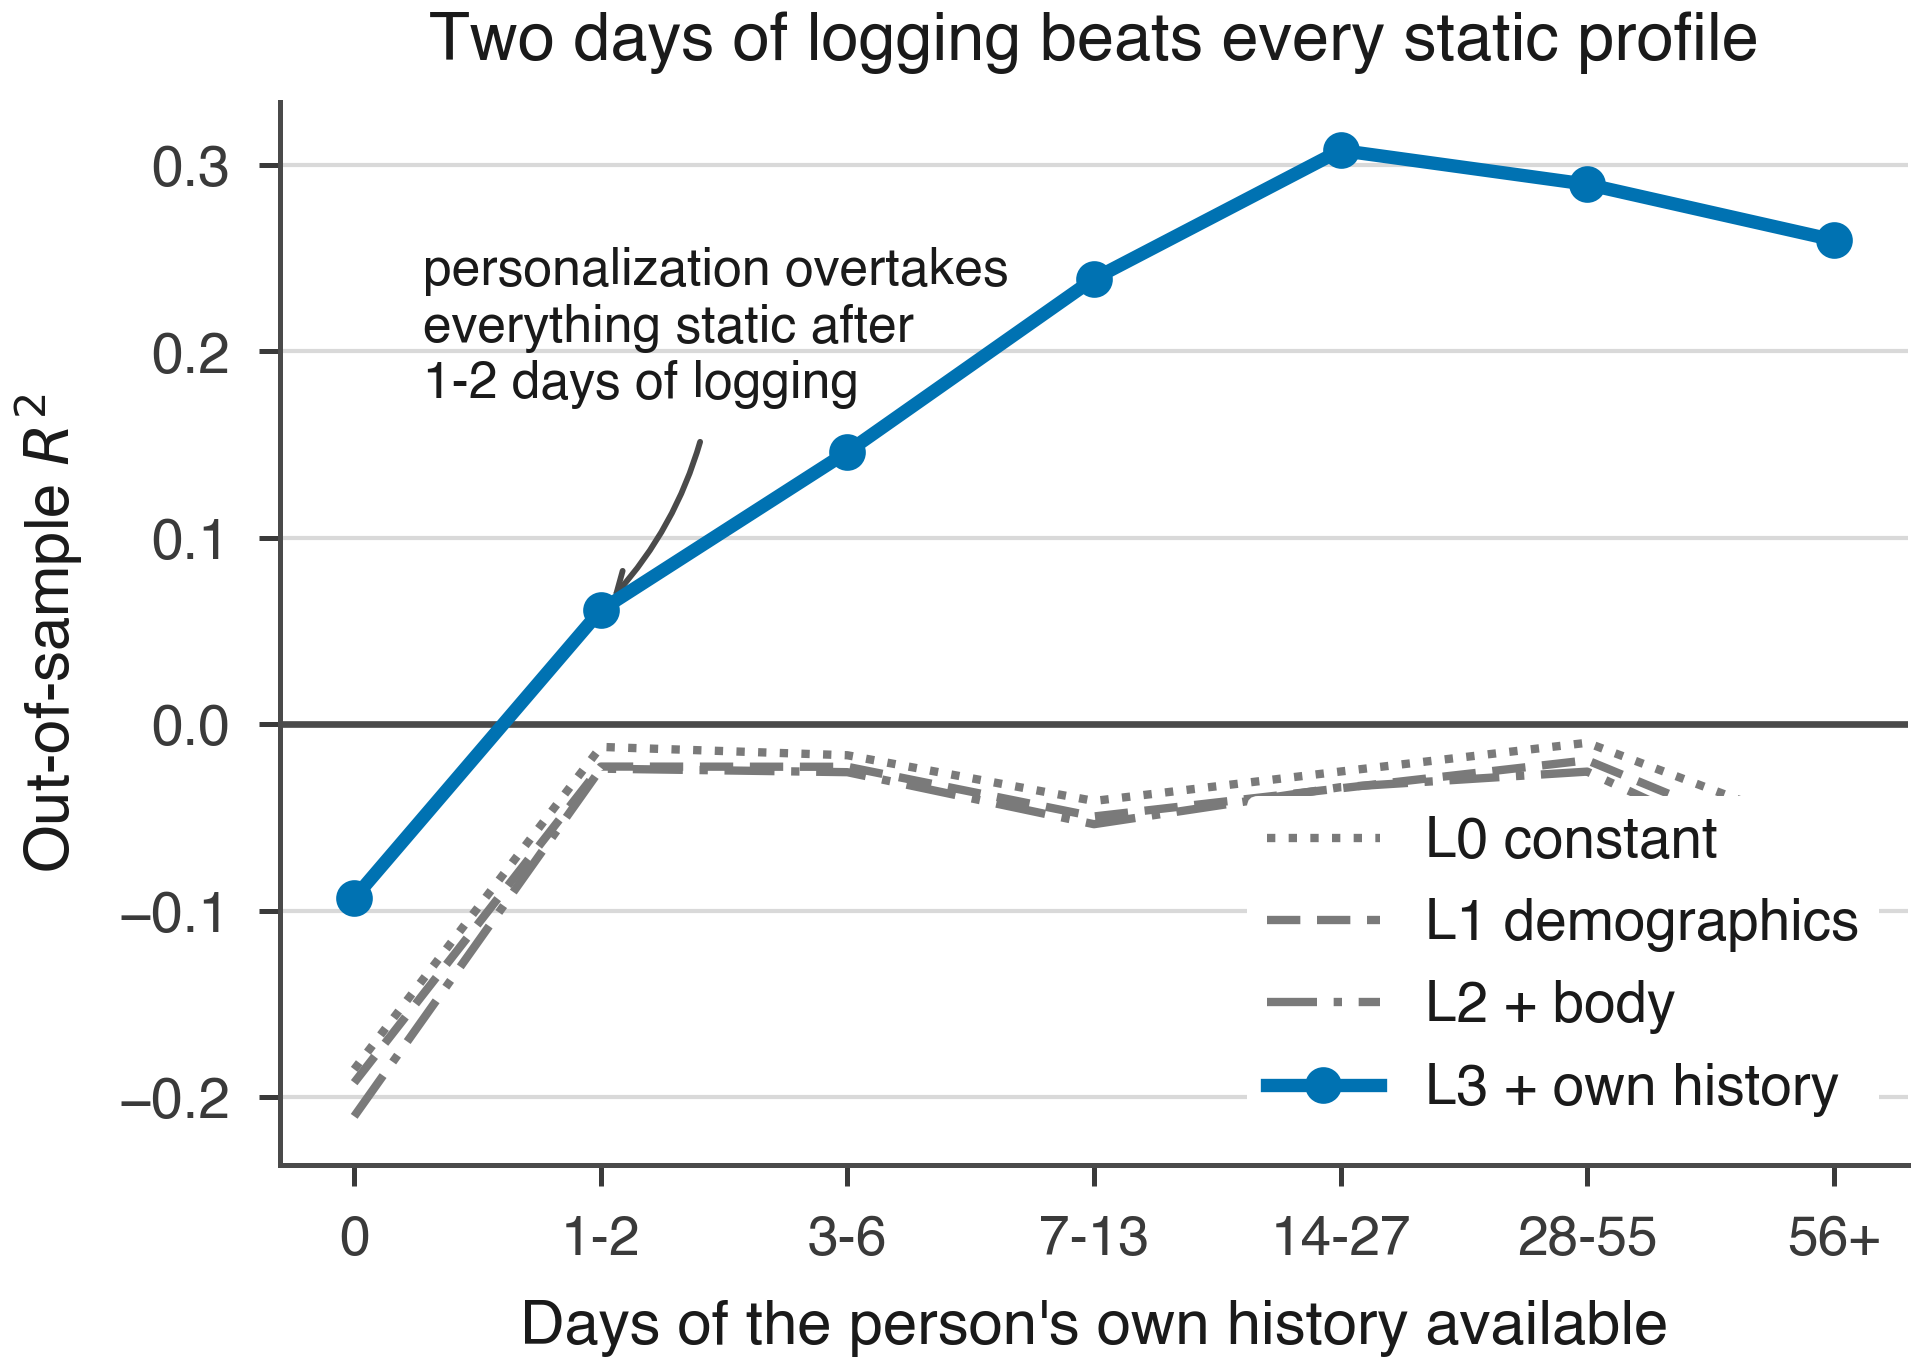
\includegraphics[width=\columnwidth]{f09_coldstart.png}
\caption{Personalization as a function of accumulated history, leave-one-person-out. One to two days of logging already beats every static rung.}
\label{fig:coldstart}
\end{figure}

With zero days, L3 is $-0.093$ and nothing works. With one to two days it is $+0.061$, already above every static rung. Seven to thirteen days gives $+0.239$ and the curve peaks at $+0.308$ between fourteen and twenty-seven days. Beyond that it declines mildly, to $+0.260$ past fifty-six days. We flag that decline as unexplained: it may be behavioural drift over a long study, or it may be that people who log for eight weeks are a different and harder subset. With 71 participants we cannot separate those and do not claim to.

The practical consequence is that the cold-start window is days, not months. An application should run the knowledge layer for the first few days and switch on personalization almost immediately.

%========================================
\section{An Architecture, and What to Collect}

\subsection{Three Layers}
The results imply a specific division of labour (Fig.~\ref{fig:arch}). Demographics do not predict behaviour, but they determine what is \textit{safe}: heart-rate zones, screening questions, contraindications, and nutritional targets that vary by age and sex. The finding is therefore sharper than "demographics are useless". Demographics tell you what is permissible for somebody and almost nothing about what they will do. A recommender needs both, from different sources.

\begin{figure*}[t]
\centering
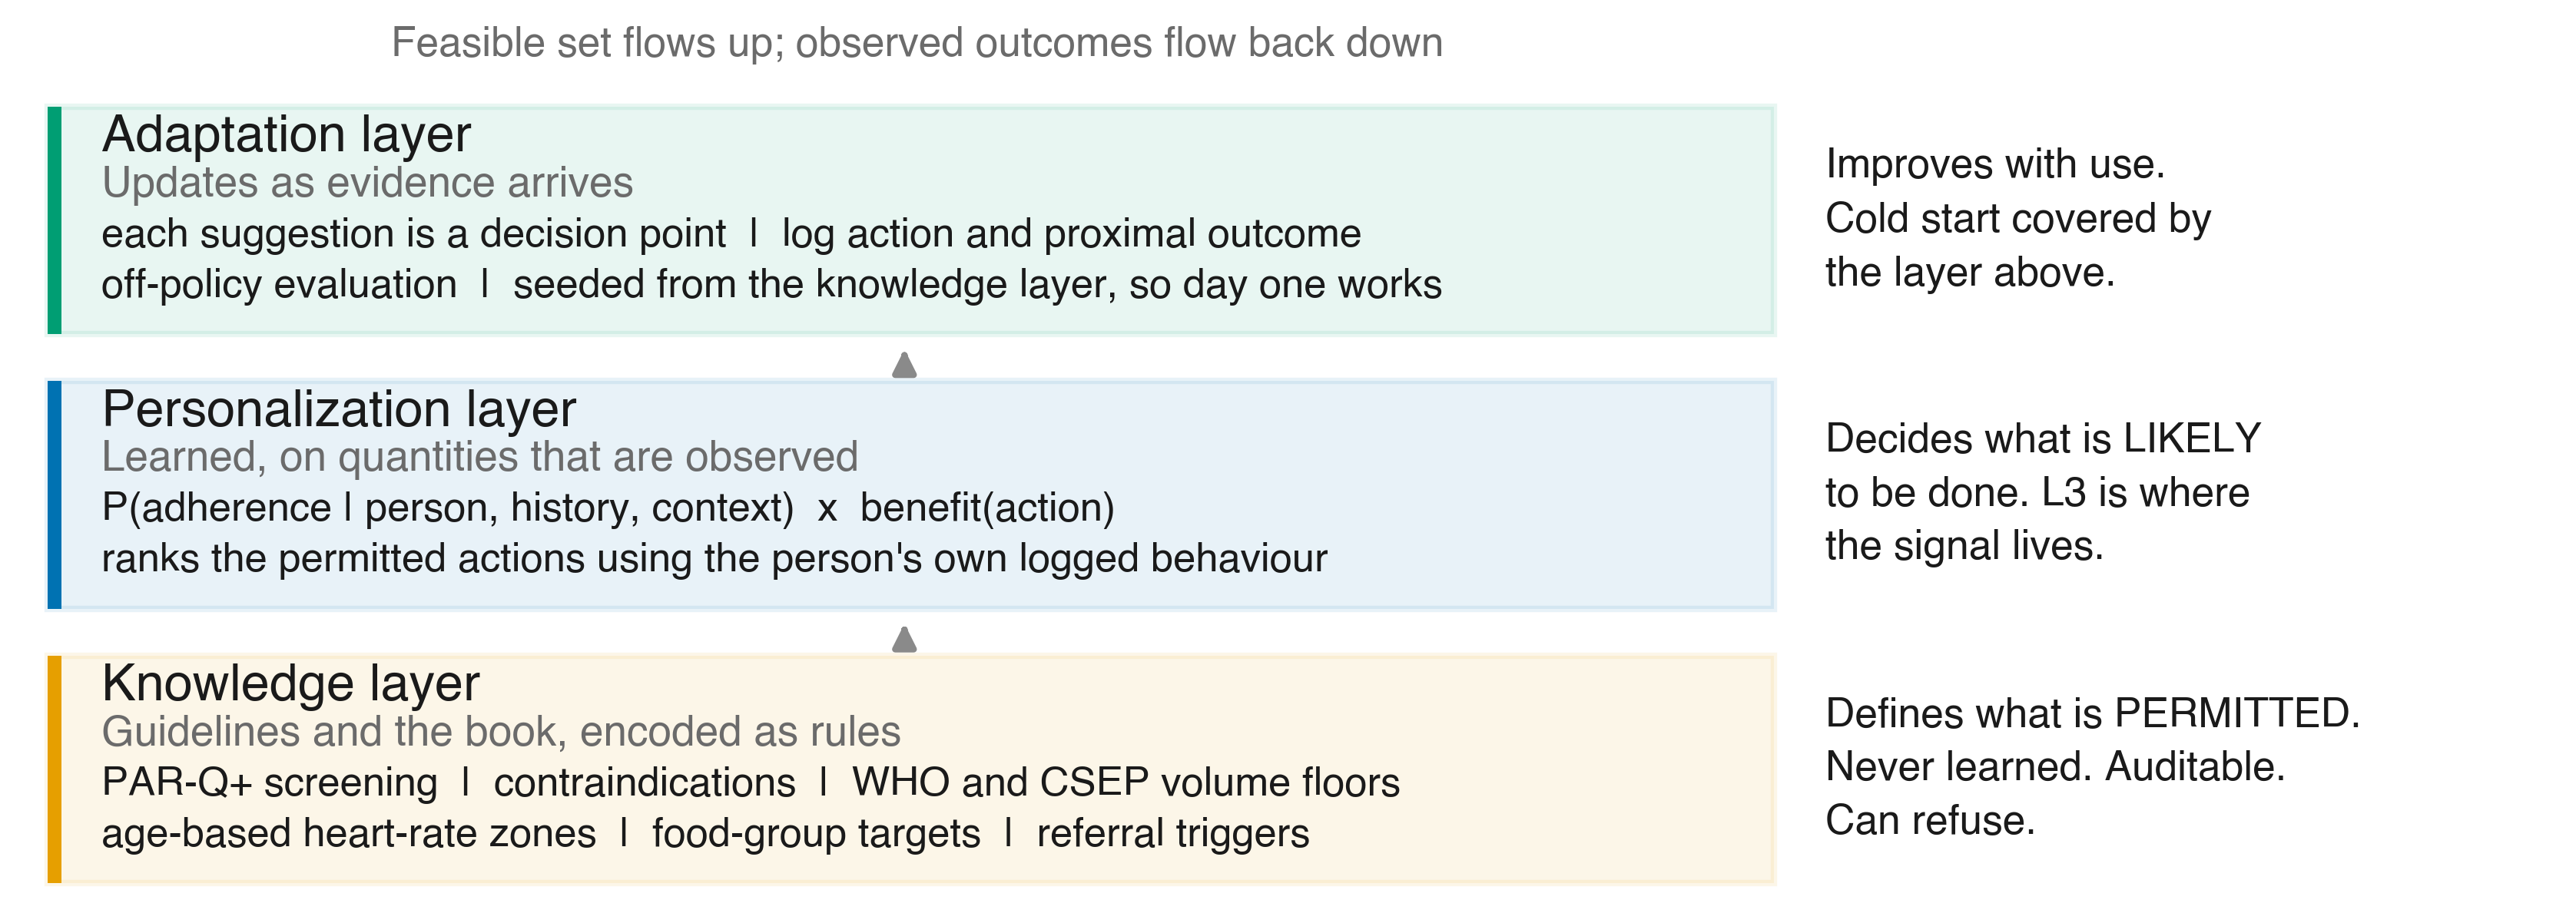
\includegraphics[width=\textwidth]{f12_architecture.png}
\caption{The architecture implied by the measurements. Expert knowledge defines what is permitted and can refuse; learned models rank the permitted actions using the person's own history; adaptation improves with use.}
\label{fig:arch}
\end{figure*}

\subsection{The Privacy-Utility Curve}
Each rung costs more disclosure than the one below, so measuring benefit per rung is simultaneously measuring the price of that benefit (Fig.~\ref{fig:privacy}).

\begin{figure}[t]
\centering
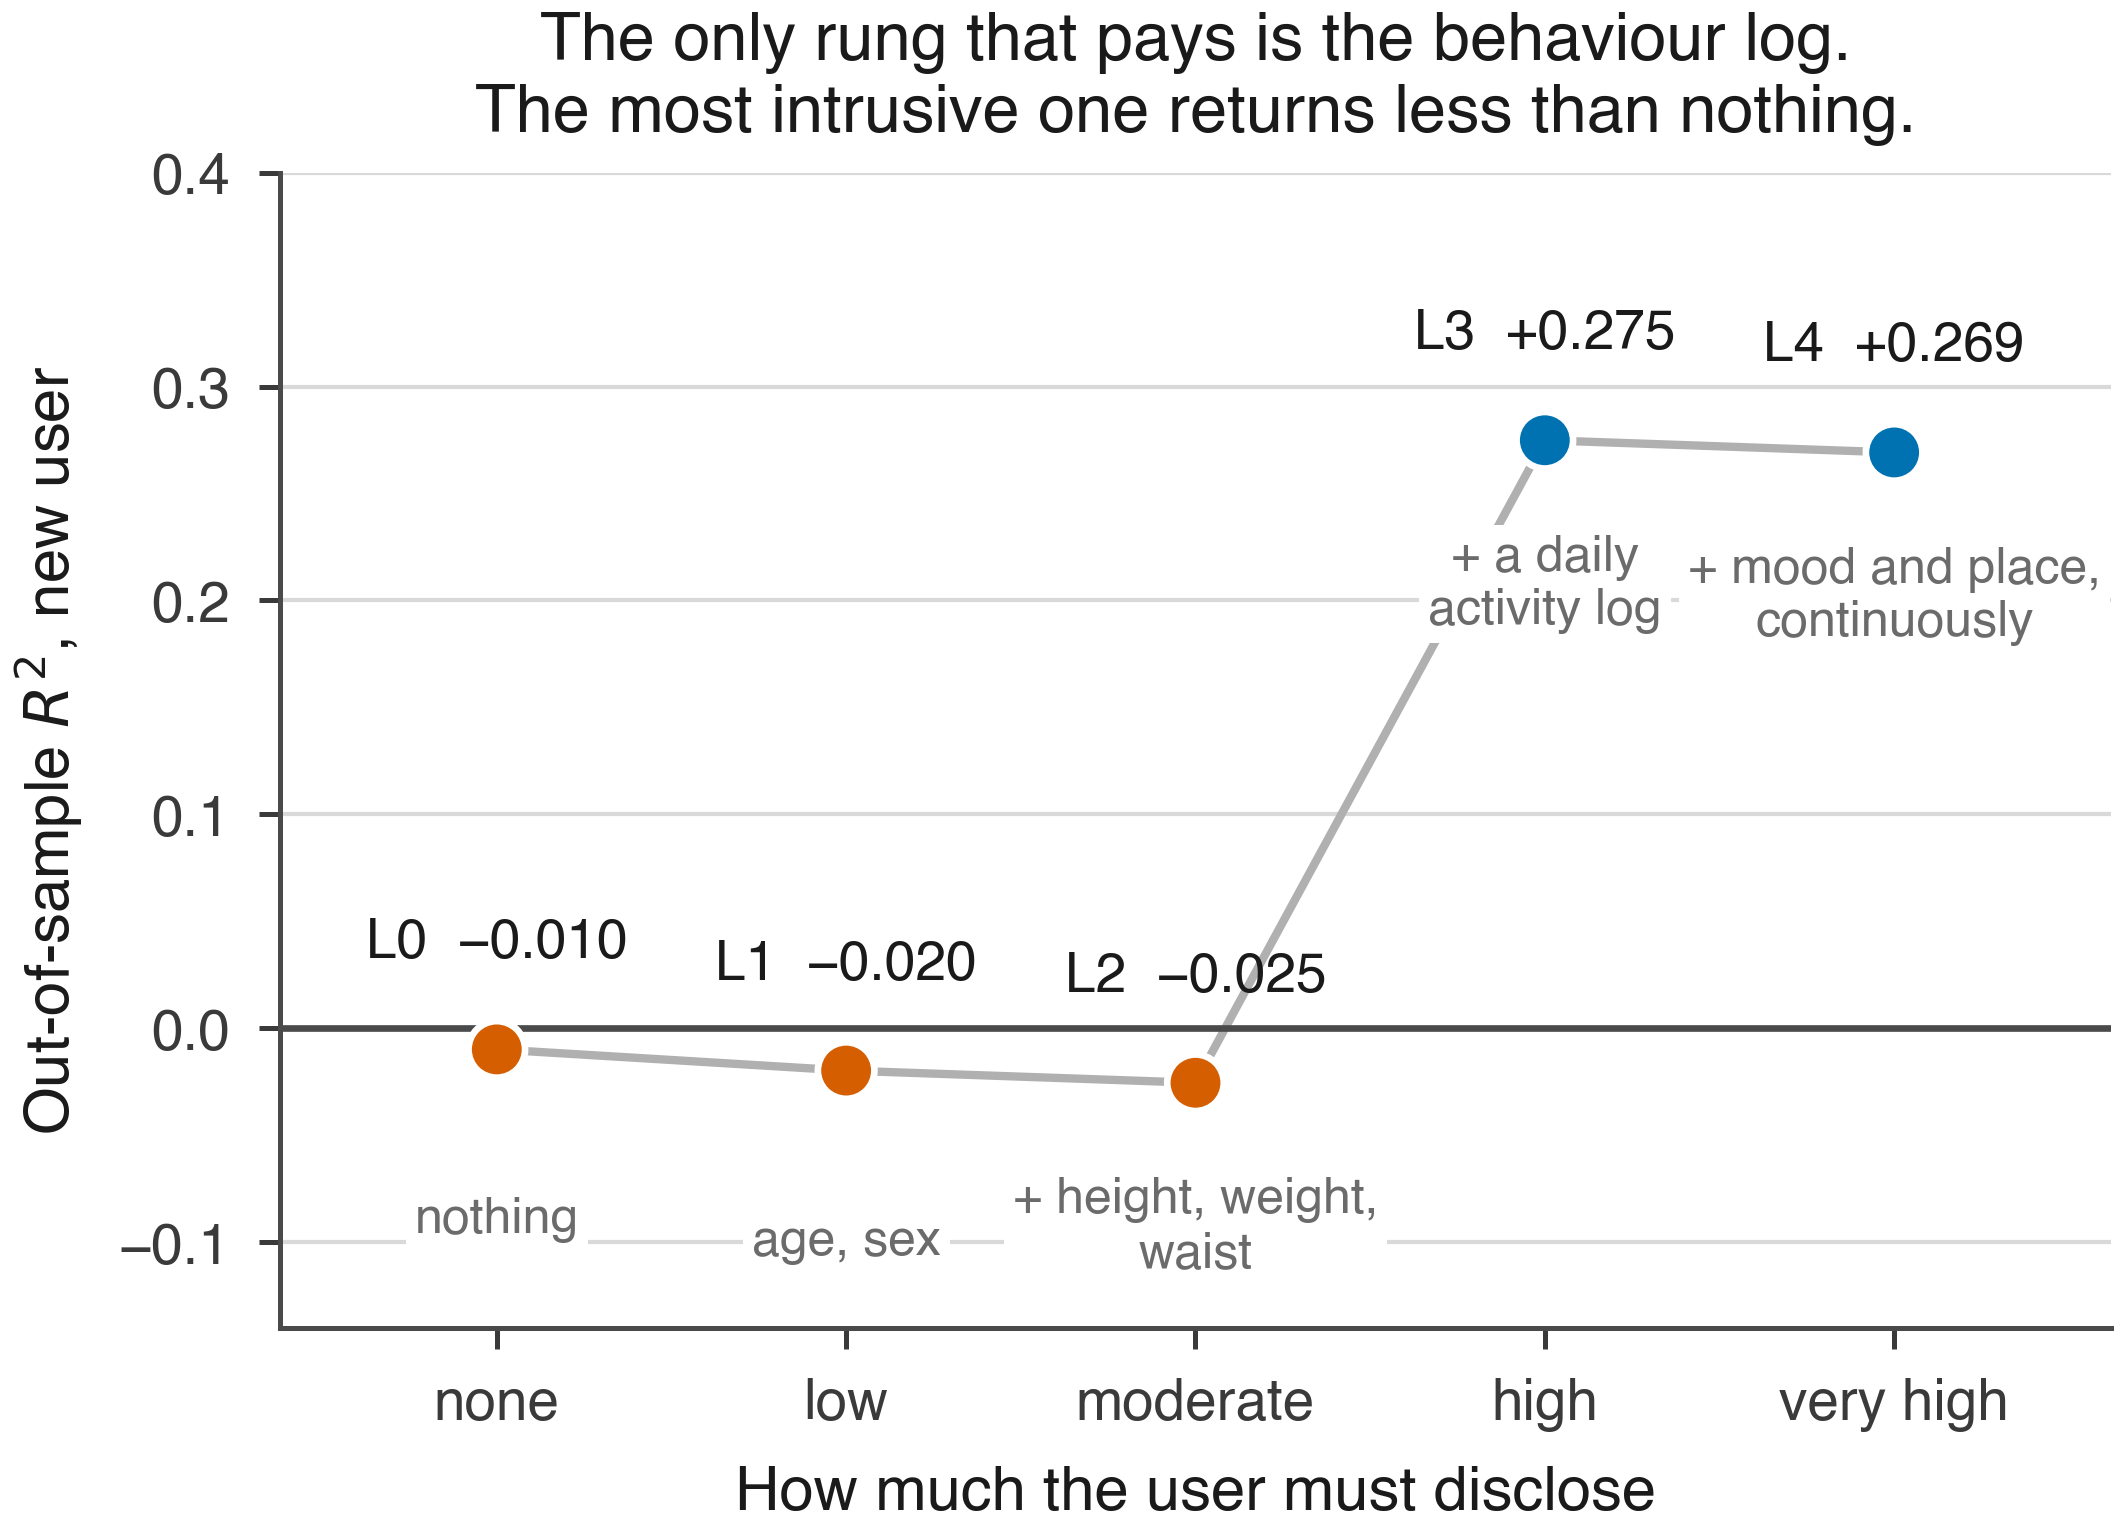
\includegraphics[width=\columnwidth]{f10_privacy_utility.png}
\caption{Benefit against disclosure for a new user. Three of four marginal gains are negative. The only rung that pays for itself is a behaviour log.}
\label{fig:privacy}
\end{figure}

For a new user, L0 gives $-0.0099$, L1 $-0.0198$, L2 $-0.0255$, L3 $+0.2749$, and L4 $+0.2692$. The paired cluster-bootstrap marginal gains are $-0.0099$ $[-0.014, -0.006]$, $-0.0057$ $[-0.013, +0.001]$, $+0.3004$ $[+0.209, +0.401]$, and $-0.0048$ $[-0.010, -0.000]$. One gain is large and unambiguous, the move to a behaviour log. The two negative gains that exclude zero do so by hundredths of a point, which is a real but negligible penalty for adding uninformative predictors to a fitted model rather than evidence that disclosure harms anyone. The practical reading is that one rung pays and the others do not.

This is data minimization argued from evidence. The usual privacy argument promises to handle sensitive data carefully. The stronger argument, available here, is that the sensitive data is not needed.

\subsection{Obtaining the Data Responsibly}
The rung that does pay, a daily behaviour log, is still personal health information, and collecting it imposes obligations. We set out the design we would deploy.

\textbf{Purpose-bound, revocable consent.} Consent is requested per data category at the moment that category first earns its place, not as a single blanket agreement at signup. Declining or later withdrawing must degrade the system to a lower rung rather than break it, which is feasible precisely because the rungs are separable.

Mobile health applications have a poor record on data sharing \cite{tangari2021bmj, papageorgiou2018privacy}, which raises the bar for anyone adding a new collection stream.

\textbf{Compute where the data lives.} The L3 features are per-person summaries: trailing means, variability, day-of-week deviation, and recent adherence. All are computable on the user's own device, so raw logs need never leave it. Only the shared coefficients require pooling, which is the setting federated learning was designed for \cite{rieke2020federated}.

\textbf{Least-privilege storage.} Row-level security so a record is readable only by the person it belongs to, encryption in transit and at rest, and identifiers stored separately from measurements.

\textbf{Retention and deletion.} A stated retention window, deletion on request, and an explicit policy for what happens to a fitted model when somebody withdraws.

\textbf{Regulatory and ethical frame.} An application deployed from British Columbia falls under PIPEDA \cite{pipeda2000} and BC PIPA, and the GDPR \cite{gdpr2016} where there are European users, whose data-minimization principle this section argues from evidence rather than from principle. The present study uses only public, de-identified secondary data and required no ethics review. Deploying a recommender to real users, or conducting a trial within the application, would require research ethics board approval under TCPS 2 \cite{tcps2022}, and we state that here so the boundary is not blurred.

\textbf{Refusal.} The system advises on behaviour and does not diagnose. The book's own referral triggers, including chest pain during exercise, persistently elevated resting heart rate, unexplained weight change, and suspected depression, are encoded as hard gates that stop recommendation and defer to a clinician.

%========================================
\section{Limitations}

The longitudinal evidence rests on 71 people in one cohort with 33 in a second, which is small, and both are convenience samples of device owners rather than representative populations. Adherence is measured on a binned goal, as declared in Section~\ref{sec:adherence}. The NHANES activity measure is self-reported and covers recreational and occupational domains through a questionnaire rather than accelerometry. Our L4 rung is a simplified proxy for context, using yesterday's mood, place, and physiology; a full JITAI with randomized decision points could plausibly extract more, and our negative result for L4 should be read as applying to this operationalization at this sample size, not as a refutation of context-aware intervention in general. The decline in L3 performance beyond eight weeks is unexplained. Finally, and most importantly, all results concern short-horizon behaviour prediction and adherence. We do not measure health outcomes, and better prediction does not entail better behaviour change. The evidence on that point is genuinely mixed. In a four-month factorial trial, static goals produced a larger average increase in daily steps than adaptive goals derived from a participant's own recent history (2{,}630 versus 2{,}149 steps per day), although the difference was not significant ($p = 0.095$), the adaptive arm decayed more slowly, and the authors conclude in favour of adaptive goals \cite{adams2017goals}; a later twelve-month trial also favoured them \cite{adams2022reinforcement}. Knowing what somebody will do is not the same as knowing what to ask of them, and this paper establishes only the first.

%========================================
\section{Conclusion}

Bodies are stable and behaviour is not, and that single fact organizes the design of a health recommender. Static profiles, including the guideline-faithful engine written by a domain expert for the book this work accompanies, predict the body extremely well and predict behaviour at or below the level of an uninformative guess. The variance decomposition explains why: roughly three quarters of what a person does is a property of the day rather than of the person, so no profile can reach it. What does reach it is the person's own recent history, which is worth $+0.24$ in $R^2$ where body measurements are worth $+0.0004$, which raises adherence prediction from AUC 0.604 to 0.746, and which becomes useful after one to two days of logging rather than months.

The practical recommendation is therefore narrow and concrete. Keep expert knowledge for what it is good at, which is deciding what is safe and permissible and when to refuse, using established screening instruments \cite{warburton2011parqplus}. Learn the rest from the person's own log. Collect that log. On this evidence the more intrusive layer did not measurably help, so the burden of proof sits with anyone proposing to collect it; we stress that our L4 tests one sparse operationalization at one sample size, and a properly randomized just-in-time design could still find value there \cite{nahumshani2018jitai, klasnja2015mrt}.


%========================================
\appendices
\section{Screening Candidate Datasets for Fabrication}
\label{app:battery}
\subsection{Why We Screened}
Public datasets advertising fitness recommendations are frequently synthetic. Of 29 candidate datasets we acquired, 5 proved fabricated. One is an 80{,}000-row file containing 16 distinct records in which the exercise and meal labels are exact functions of BMI category. A third, widely used, is 75.7\% synthesized by SMOTE \cite{chawla2002smote, palechor2019obesity}, a fact rarely mentioned by those who use it. Another advertises personalized clinical diet recommendations; we recovered its generator exactly, and the recommendation is the patient's own reported intake plus uniform noise, with a correlation between recommended calories and BMI of 0.007.

\subsection{The Four Detectors}
A single-column determination test asks whether a target is an exact function of one other column \cite{huhtala1999tane, abedjan2015profiling}. It is a cross-sectional test, and it returns a benign verdict on four of these five files. Fabrication is not one phenomenon, so we use four detectors:

\begin{itemize}
\item \textbf{D1, lookup table.} Exact single-column determination and row compression.
\item \textbf{D2, independent noise.} Best achievable predictive signal over several candidate targets under a person-grouped split. Chance-level performance everywhere means the columns were drawn independently.
\item \textbf{D3, temporal fabrication.} Within-person lag-1 autocorrelation of physiological state. A real person's resting heart rate tomorrow resembles today's.
\item \textbf{D4, internal inconsistency.} Recompute derived quantities from their components, for example BMI from height and weight.
\end{itemize}

\begin{table}[t]
\centering
\caption{Fabrication Detection. Each Detector Catches a Different Failure; No Detector Catches More Than Three of Five}
\begin{tabular}{@{}lcccc@{}}
\toprule
\textbf{Detector} & \textbf{Caught} & \multicolumn{3}{c}{\textbf{Separating evidence}} \\
\midrule
D1 lookup        & 1 of 5 & \multicolumn{3}{l}{16 distinct rows in 80{,}000} \\
D2 no signal     & 2 of 5 & \multicolumn{3}{l}{AUC 0.51 vs 0.80 on real data} \\
D3 temporal      & 3 of 5 & \multicolumn{3}{l}{lag-1 $r$ 0.12 vs 0.86 on real data} \\
D4 inconsistent  & 1 of 5 & \multicolumn{3}{l}{BMI contradicts inputs in 95.4\%} \\
\midrule
\textbf{D1 alone}      & \textbf{1 of 5} & \multicolumn{3}{l}{the published screen} \\
\textbf{Full battery}  & \textbf{5 of 5} & \multicolumn{3}{l}{0 false alarms on 4 real sets} \\
\bottomrule
\end{tabular}
\label{tab:battery}
\end{table}

Table~\ref{tab:battery} reports the outcome, Fig.~\ref{fig:matrix} shows which detector caught which dataset, and Fig.~\ref{fig:temporal} shows the temporal signature, which is the most decisive single diagnostic for panel data. D1 is the check most commonly recommended for this purpose, and its shortfall here is the reason the other three exist.

\begin{figure}[t]
\centering
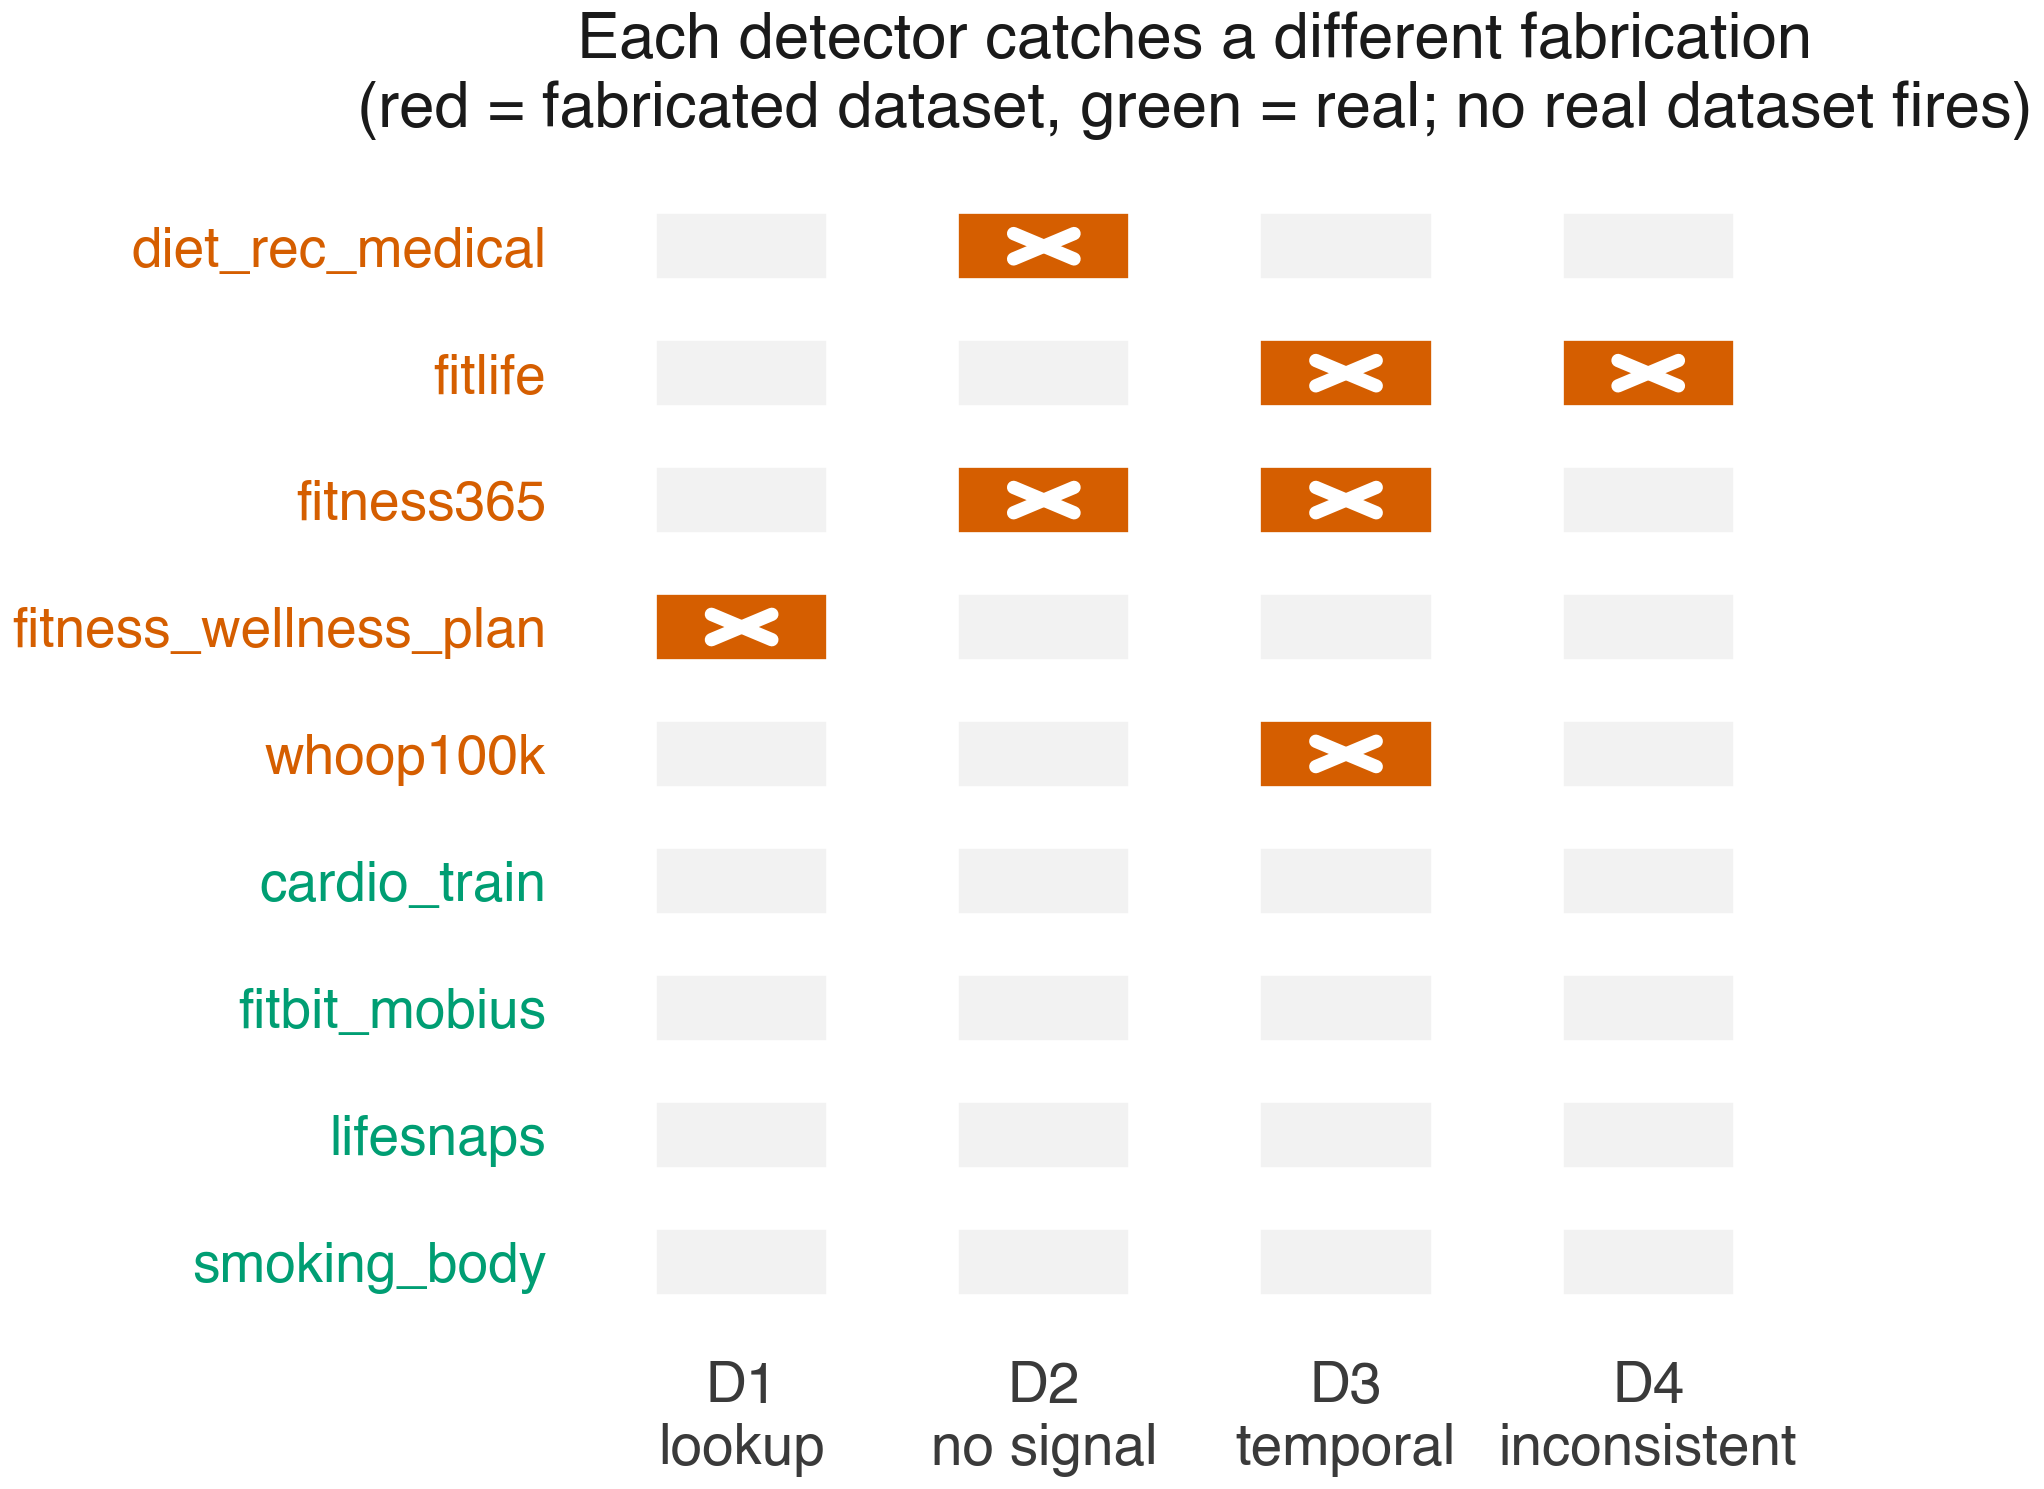
\includegraphics[width=\columnwidth]{f02_fabrication_matrix.png}
\caption{Which detector caught which dataset. No single detector catches more than three of the five fabricated files, and none fires on any of the four real ones.}
\label{fig:matrix}
\end{figure}

\begin{figure}[t]
\centering
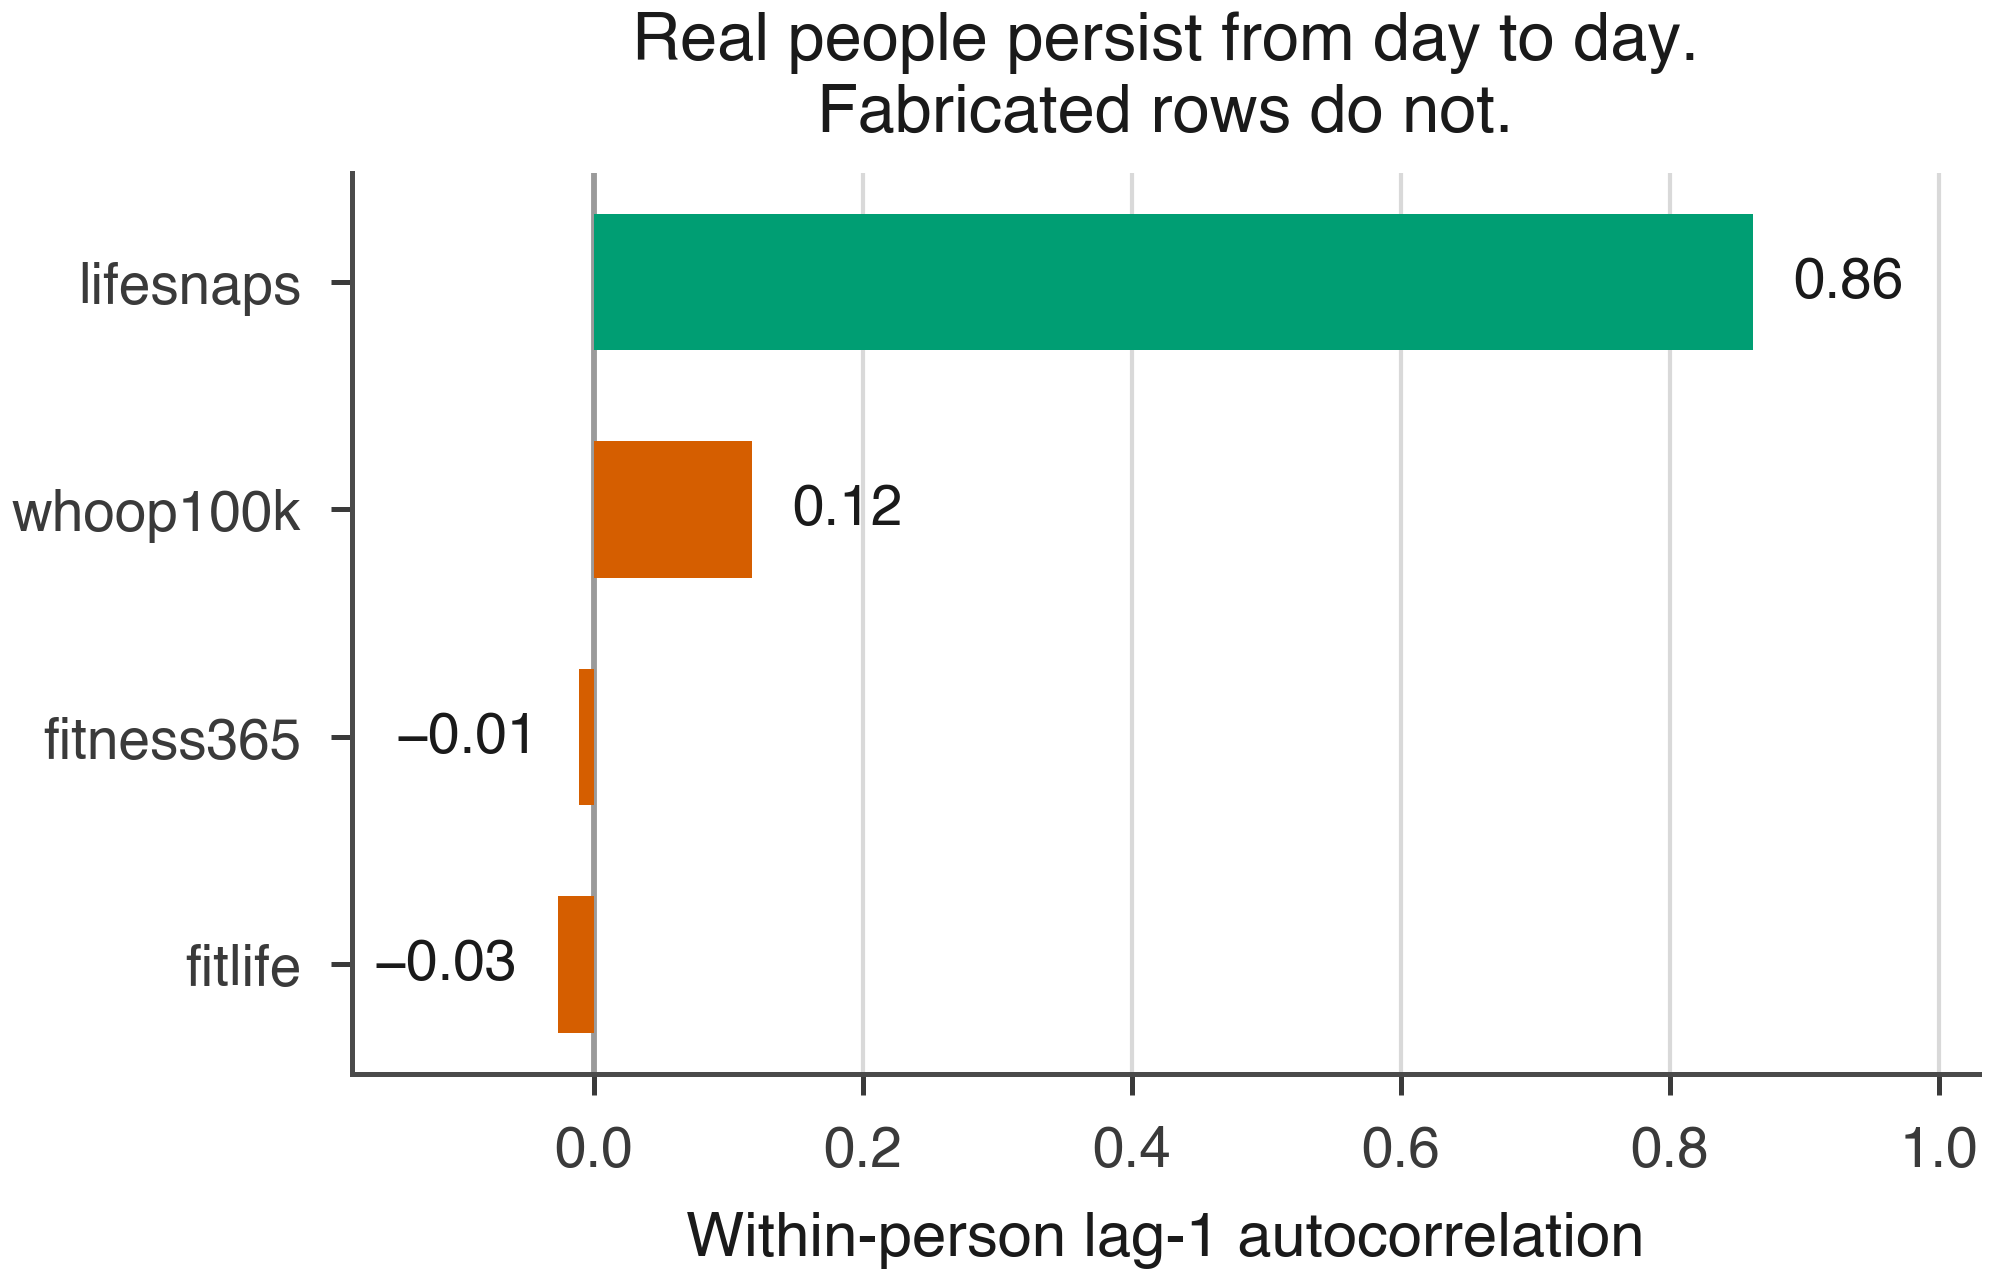
\includegraphics[width=\columnwidth]{f03_temporal_fingerprint.png}
\caption{Within-person lag-1 autocorrelation of the most persistent physiological state variable available in each dataset. Real cohorts retain the person from day to day. Fabricated files do not, because their rows were drawn independently.}
\label{fig:temporal}
\end{figure}


\section*{Reproducibility}

All experiments are seeded. The screen, the harmonized panel construction, every experiment, the figure code, and a script that re-checks each number in this paper against the committed outputs are available in the replication package accompanying this submission.

\balance
\bibliographystyle{IEEEtran}
\bibliography{references}

\end{document}
